\documentclass[12pt,a4paper]{article}
\usepackage{../.tex/mcs-notes}
\usepackage{todonotes}
\usepackage{dsfont}
% \usepackage{multicol}

\settitle
{Дискретная теория вероятностей.}
{Юрий Александрович Давыдов}
{\%D0\%94\%D0\%A2\%D0\%92/DPT.pdf}
\date{}

\newcommand{\ind}{\ensuremath{\mathds{1}}\xspace}
\newcommand{\Var}{\ensuremath{\mathrm{Var}}\xspace}
\newcommand{\cov}{\ensuremath{\mathrm{cov}}\xspace}
\newcommand{\probto}{\mathop{\stackrel{\PP}{\to}}}
\DeclareMathOperator*{\osc}{osc}
\newcommand{\Deq}{\mathop{\stackrel{\mathcal{D}}{=}}}


\begin{document}
    \maketitle

    \listoftodos[TODOs]

    \tableofcontents

    \vspace{2em}

    Литература:
    \begin{itemize}
        \item А.Н. Ширяев, ``Вероятность''.
        \item М.А. Лифшиц, ``Лекции''
        \item Ю.Г. Борисович, Н.М. Близняков, Я.А. Израилевич, Т.Н. Фоменко, ``Введение в топологию'', М.:Наука. Физматлит, 1995.
        \item James Munkres, Topology.
        \item \href{http://mathcenter.spb.ru/nikaan/book/bernstein_bio.pdf}{Биография Сергея Натановича Бернштейна}.
    \end{itemize}

    \section{Вероятностные пространства и стандартные следствия}

    \subsection{Вероятностное пространство}

    \begin{definition}
        \emph{Вероятностное пространство} --- это тройка $(\Omega, \mathcal{F}, \PP)$, где
        \begin{itemize}
            \item $\Omega \neq \varnothing$ --- множество объектов случайной природы, называемых \emph{элементарными событиями (исходами)},
            \item $\mathcal{F}$ --- сигма-алгебра над множеством $\Omega$ (т.е. такое подмножество $\mathcal{P}(\Omega)$, что
                \begin{enumerate}
                    \item $\mathcal{F}$ содержит $\Omega$,
                    \item для всякого $A \in \mathcal{F}$ множество $\Omega \setminus A$ содержится в $\mathcal{F}$,
                    \item для всякого не более чем счётного семейства $\{A_i\}_{i \in I}$ множеств из $\mathcal{F}$ множества
                        \[
                            \bigcup_{i \in I} A_i
                            \qquad \text{ и } \qquad
                            \bigcap_{i \in I} A_i
                        \]
                        содержатся в $\mathcal{F}$),
                \end{enumerate}
                которая называется множеством \emph{(случайных) событий},
            \item $\PP$ --- счётно-аддитивная мера, что $\PP(\Omega) = 1$ (т.е. функция из $\mathcal{F}$ в $[0; 1]$, что
                \begin{enumerate}
                    \item $\PP(\varnothing) = 0$, $\PP(\Omega) = 1$,
                    \item для всякого не более чем счётного семейства $\{A_i\}_{i \in I}$ дизъюнктных множеств из $\mathcal{F}$
                        \[\PP\left(\bigcup_{i \in I} A_i\right) = \sum_{i \in I} \PP(A_i);\]
                \end{enumerate}
                значение $\PP(A)$ называется \emph{вероятностью события $A$}).
        \end{itemize}
    \end{definition}

    \begin{example}
        Пусть мы бросаем монетку (один раз).
        \begin{enumerate}
            \item Тогда множество исходов будет состоять из элементарных событий ``выпал орёл'' и ``выпала решка'':
                \[\Omega := \{\text{Орёл}; \text{Решка}\}\]
            \item Множество событий будет состоять из событий:
                \begin{enumerate}
                    \item $\varnothing$ --- ничего не выпало, т.е. ничего не произошло,
                    \item $\{\text{Орёл}\}$ --- выпал орёл,
                    \item $\{\text{Решка}\}$ --- выпала решка,
                    \item $\{\text{Орёл}; \text{Решка}\}$ --- выпал орёл или решка, т.е. что-то произошло.
                \end{enumerate}
                Т.е. в данном случае $\mathcal{F} = \mathcal{P}(\Omega)$.
            \item Понятно, что
                \[
                    \PP(\varnothing) = 0,
                    \quad \text{ а } \quad
                    \PP(\{\text{Орёл}; \text{Решка}\}) = 1.
                \]
                При этом для всякой величины $p \in [0; 1]$ может быть, что
                \[
                    \PP(\{\text{Орёл}\}) = p,
                    \quad \text{ а } \quad
                    \PP(\{\text{Решка}\}) = 1 - p.
                \]
                В случае $p = \frac{1}{2}$ монетку называют \emph{симметричной} (иначе \emph{несимметричной}).
        \end{enumerate}
    \end{example}

    \begin{remark*}[``стабилизация частот'']
        Пусть мы проводим один и тот же эксперимент $n$ раз и смотрим, сколько раз реализовалось событие $A$. Обозначим это количество реализаций за $\nu_n(A)$. При этом если эксперимент брать ``реальным'', например, взятым из физики (подбрасывание монеты, бросание игрального кубика, etc.), то можно заметить следующие явления.
        \begin{enumerate}
            \item (эмпирический факт) Для всякого события $A$ имеет место сходимость
                \[\lim_{n \to \infty} \frac{\nu_n(A)}{n} = P(A).\]
                Это и хочется назвать вероятностью.
            \item Если $A = \Omega$, то $\nu_n(A)$ должно ровняться $n$, а значит
                \[P(A) = \lim_{n \to \infty} \frac{\nu_n(A)}{n} = 1.\]
                А если $A = \varnothing$, то $P(A) = 0$.
            \item Для всякого события $A$ верно, что $\nu_n(A) \in [0; n]$. Следовательно $P(A) \in [0; 1]$.
            \item Если события $A$ и $B$ дизъюнктны, то $\nu_n(A) + \nu_n(B) = \nu_n(A \cup B)$. Отсюда следует аддитивность вероятности; и по аналогии получается счётная аддитивность.
        \end{enumerate}
    \end{remark*}

    \begin{lemma}\ 
        \begin{enumerate}
            \item Для всяких событий $A$ и $B$
                \[A \subseteq B \quad \Longrightarrow \quad \PP(A) \leqslant \PP(B).\]
            \item Для всякого события $A$
                \[\PP(A) + \PP(A^C) = 1,\]
                где $A^C := \Omega \setminus A$.
            \item Для всяких событий $A$ и $B$
                \[\PP(A \cup B) = \PP(A) + \PP(B) - \PP(A \cap B).\]
            \item Для всякого не более чем счётного семейства событий $\{A_i\}_{i \in I}$
                \[\PP\left(\bigcup_{i \in I} A_i\right) \leqslant \sum_{i \in I} \PP(A_i),\]
                и равенство достигается только если $\PP(A_i \cap A_j) = 0$ для всех $i \neq j$.
            \item Для всякой последовательности вложенных событий $\{A_n\}_{n=0}^\infty$ ($A_{n+1} \supseteq A_n$)
                \[\PP\left(\bigcap_{n=0}^\infty A_n\right) = \lim_{n \to \infty} \PP(A_n).\]
            \item Для всякой последовательности вложенных событий $\{A_n\}_{n=0}^\infty$ ($A_{n+1} \subseteq A_n$)
                \[\PP\left(\bigcap_{n=0}^\infty A_n\right) = \lim_{n \to \infty} \PP(A_n).\]
        \end{enumerate}
    \end{lemma}

    \begin{definition}
        Вероятностное пространство $(\Omega, \mathcal{F}, \PP)$ называется \emph{дискретным}, если $\Omega$ не более чем счётно, а $\mathcal{F} = \mathcal{P}(\Omega)$.
    \end{definition}

    \begin{theorem}
        Пусть даны не более чем счётное $\Omega$ и $\mathcal{F} = \mathcal{P}(\Omega)$.
        \begin{enumerate}
            \item Пусть $(\Omega, \mathcal{F}, \PP)$ --- дискретное вероятностное пространство. Для всякого $\omega \in \Omega$ можно обозначить
                \[p_\omega := \PP(\omega).\]
                Тогда
                \begin{enumerate}
                    \item каждое $p_\omega \geqslant 0$,
                    \item
                        \[\sum_{\omega \in \Omega} p_\omega = 1.\]
                \end{enumerate}
                И при этом $\PP$ можно задать условием
                \[\PP(A) = \sum_{\omega \in A} p_\omega\]
            \item Пусть для всякого $\omega \in \Omega$ определено вещественное $p_\omega$, что
                \begin{enumerate}
                    \item каждое $p_\omega \geqslant 0$,
                    \item
                        \[\sum_{\omega \in \Omega} p_\omega = 1.\]
                \end{enumerate}
                Тогда можно задать функцию $\PP: \mathcal{F} \to [0; 1]$ условием
                \[\PP(A) = \sum_{\omega \in A} p_\omega,\]
                и тогда $(\Omega, \mathcal{F}, \PP)$ будет дискретным вероятностным пространством.
        \end{enumerate}
    \end{theorem}

    \begin{proof}
        \begin{enumerate}
            \item Действительно:
                \begin{enumerate}
                    \item Каждое
                        \[p_\omega = \PP(\omega) \geqslant 0.\]
                    \item Поскольку $\Omega = \bigsqcup_{\omega \in \Omega} \{\omega\}$, то
                        \[\sum_{\omega \in \Omega} p_\omega = \sum_{\omega \in \Omega} \PP(\omega) = \PP(\Omega) = 1.\]
                \end{enumerate}
                И аналогично $A = \bigsqcup_{\omega \in A} \{\omega\}$, а значит
                \[\PP(A) = \sum_{\omega \in A} \PP(\omega) = \sum_{\omega \in A} p_\omega.\]
            \item Действительно, если $A = \bigsqcup_{i \in I} A_i$ ($I$ не более чем счётно), то (так как каждое $A_i$ не более чем счётно)
                \[\PP(A) = \sum_{\omega \in A} p_\omega = \sum_{i \in I} \sum_{\omega \in A_i} p_\omega = \sum_{i \in I} \PP(A_i)\]
                (так как мы рассуждаем в рамках абсолютно сходящегося ряда). Ну и, конечно,
                \[
                    \PP(\varnothing) = \sum_{\omega \in \varnothing} p_\omega = 0
                    \qquad \text{ и } \qquad
                    \PP(\Omega) = \sum_{\omega \in \Omega} p_\omega = 1
                \]
        \end{enumerate}
    \end{proof}

    \begin{definition}
        $(\Omega, \mathcal{F}, \PP)$ называется \emph{пространством классического типа}, если $\Omega$ кончено, $\mathcal{F} = \mathcal{P}(\Omega)$ и для всякого $\omega \in \Omega$
        \[\PP(\omega) = \frac{1}{|\Omega|}.\]
    \end{definition}

    \begin{remark}
        В классическом пространстве соответственно имеем, что
        \[\PP(A) = \frac{|A|}{|\Omega|}\]
    \end{remark}

    \subsection{Условная вероятность}

    \begin{definition}
        \emph{Вероятность события $A$ при условии события $B$} (где $\PP(B) \neq 0$) есть
        \[\PP_B(A) = \PP(A \mid B) := \frac{\PP(A \cap B)}{\PP(B)}.\]
    \end{definition}

    \begin{theorem}
        Пусть даны вероятностное пространство $(\Omega, \mathcal{F}, \PP)$ и $B \in \mathcal{F}$, что $\PP(B) \neq 0$. Тогда тройки $(\Omega, \mathcal{F}, P)$ и $(B, \mathcal{F}_B, P_B)$, где
        \[\mathcal{F}_B := \{S \in \mathcal{F} \mid S \subseteq B\},\]
        а
        \[P: \mathcal{F} \to [0; 1], A \mapsto \frac{\PP(A \cap B)}{\PP(B)}\]
        и
        \[P: \mathcal{F}_B \to [0; 1], A \mapsto \frac{\PP(A)}{\PP(B)},\]
        являются вероятностными пространствами.
    \end{theorem}

    \begin{proof}
        Понятно, что
        \[P(\varnothing) = 0 \qquad \text{ и } \qquad P(\Omega) = 1.\]
        Также если $A = \bigsqcup_{i \in I} A_i$ (где $I$ не более чем счётно), то
        \[
            \left(\bigcup_{i \in I} A_i \right) \cap B = \bigcup_{i \in I} A_i \cap B
            \quad \Longrightarrow \quad
            \PP\left(\left(\bigcup_{i \in I} A_i \right) \cap B\right) = \sum_{i \in I} \PP(A_i \cap B).
        \]
        Значит первая тройка является вероятностным пространством.

        Заметим, что отношение $\sim$ на $\mathcal{F}$, заданное условием
        \[S \sim T \quad \Longleftrightarrow \quad S \cap B = T \cap B\]
        определяет классы эквивалентности, минимальные по включению предстаители которых (представителем $[A]$ будет $A \cap B$), образуют $\mathcal{F}_B$. При этом для всяких $S$ и $T$ из $S \sim T$ следует, что
        \[\PP(S \cap B) = \PP(T \cap B).\]
        Также несложно понять, что $\mathcal{F}_B$ будет сигма-алгеброй. Значит $P_B$ сужением $P$ на $\mathcal{F}$ с тем же множеством значений. Таким образом вторая тройка тоже будет вероятностным пространством.
    \end{proof}

    \begin{lemma}[формула полной вероятности]
        Пусть дано не более чем счётное разбиение $\{B_i\}_{i \in I}$ множества $\Omega$ на множества из $\mathcal{F}$. Тогда для всякого события $A$
        \[\PP(A) = \sum_{i \in I} \PP(B_i) \PP(A \mid B_i).\]
    \end{lemma}

    \begin{proof}
        Поскольку $\{B_i \cap A\}_{i \in I}$ есть разбиение $A$, значит
        \[\PP(A) = \sum_{i \in I} \PP(A \cap B_i) = \sum_{i \in I} \PP(B_i) \PP(A \mid B_i)\]
    \end{proof}

    \begin{lemma}[формула Байеса]
        Для всяких событий $A$ и $B$
        \[\PP(A \mid B) = \frac{\PP(A)\PP(B \mid A)}{\PP(B)}\]
    \end{lemma}

    \begin{proof}
        \[\PP(A \mid B) = \frac{\PP(A \cap B)}{\PP(B)} = \frac{\PP(A)\PP(B \mid A)}{\PP(B)}.\]
    \end{proof}

    \begin{corollary}
        Пусть дано не более чем счётное разбиение $\{B_i\}_{i \in I}$ множества $\Omega$ на множества из $\mathcal{F}$. Тогда для всякого события $A$ и индекса $j \in I$
        \[\PP(B_j \mid A) = \frac{\PP(B_j) \mid(A \mid B_j)}{\sum_{i \in I} \PP(B_i) \PP(A \mid B_i)}.\]
    \end{corollary}

    \begin{lemma}[формула умножения]
        Для всяких событий $\{A_k\}_{i=1}^n$. Тогда
        \[\PP\left(\bigcap_{k=1}^n A_i\right) = \prod_{k=1}^n \PP\left(A_k \mid \bigcap_{i=1}^{k-1} A_i\right) = \PP(A_1) \cdot \PP(A_2 \mid A_1) \cdot \dots \cdot \PP\left(A_n \mid \bigcap_{i=1}^{n-1} A_i\right)\]
    \end{lemma}

    \subsection{Независимые события}

    \begin{definition}
        События $A$ и $B$ называются \emph{независимыми}, если
        \[\PP(A \cap B) = \PP(A) \PP(B)\]
    \end{definition}

    \begin{lemma}
        Для любых двух событий $A$ и $B$ TFAE
        \begin{enumerate}
            \item $A$ и $B$ независимы и их вероятности $>0$,
            \item $\PP(A) = \PP(A \mid B)$ (а $\PP(B) = \PP(B \mid A)$).
        \end{enumerate}
    \end{lemma}

    \begin{definition}
        Семейство событий $\{A_i\}_{i \in I}$ называется \emph{независимым} (или также \emph{``независимым в совокупности''} или \emph{``совместно независимым''}), если для всякого конечного $S \subseteq I$ верно равенство
        \[\PP\left(\bigcap_{i \in I} A_i\right) = \prod_{i \in I} \PP(A_i).\]
    \end{definition}

    \begin{remark}
        Независимость (в совокупности) есть частный случай попарной независимости (что понятно, из определения), но не является равносильным ему свойством.
    \end{remark}

    \begin{example}[пирамида Бернштейна]
        Рассмотрим пространство классического типа с $\Omega = \{1; 2; 3; 4\}$. Пусть
        \[A_1 := \{1; 4\}, \qquad A_2 := \{2; 4\} \qquad \text{ и } \qquad A_3 := \{3; 4\}.\]
        Тогда
        \[\PP(A_i) = \frac{1}{2}, \qquad \PP(A_i \cap A_j) = \frac{1}{4} = \PP(A_i) \cdot \PP(A_j) \qquad \text{ и } \qquad \PP(A_1 \cap A_2 \cap A_3) = \frac{1}{4} = \PP(A_1) \cdot \PP(A_2) \cdot \PP(A_3).\]
        Отсюда, например, следует, что
        \[\PP(A_3 \mid A_1 \cap A_2) \neq \PP(A_3)\]
    \end{example}

    \begin{theorem}
        Пусть даны некоторые натуральные $\{m_i\}_{i=1}^n$ и семейство независимых событий
        \[\{A_{i, j}\}_{\substack{i \in \{1; \dots; n\}\\ j \in \{1; \dots; m_i\}}}.\]
        Тогда семейство событий
        \[\left\{\bigcup_{j = 1}^{m_i} A_i\right\}_{i=1}^n\]
        независимо.
    \end{theorem}

    \begin{proof}
        \begin{lemma}
            Пусть дано семейство независимых событий $\{A_i\}_{i \in I} \cup \{B; C\}$. Тогда семейства
            \[\{A_i\}_{i \in I} \cup \{B \cap C\} \qquad \text{ и } \qquad \{A_i\}_{i \in I} \cup \{B \cup C\}\]
            являются независимыми (сами для себя, а не друг для друга).
        \end{lemma}

        \begin{proof}
            \begin{enumerate}
                \item Покажем для пересечения. Пусть $S \subseteq I$ --- конечное подмножество. Тогда
                    \[
                        \PP\left((B \cap C) \cap \bigcap_{i \in S} A_i\right)
                        = \PP(B) \cdot \PP(C) \cdot \prod_{i \in S} \PP(A_i)
                        = \PP(B \cap C) \cdot \prod_{i \in S} \PP(A_i).
                    \]
                    Значит
                    \[\{A_i\}_{i \in I} \cup \{B \cap C\},\]
                    действительно, независим.
                \item Покажем для объединения. Пусть $S \subseteq I$ --- конечное подмножество. Тогда
                    \begin{align*}
                        \PP\left((B \cup C) \cap \bigcap_{i \in S} A_i\right)
                        &= \PP\left(B \cap \bigcap_{i \in S} A_i\right) + \PP\left(C \cap \bigcap_{i \in S} A_i\right) - \PP\left((B \cap C) \cap \bigcap_{i \in S} A_i\right)\\
                        &= \PP(B) \cdot \prod_{i \in S} \PP(A_i) + \PP(C) \cdot \prod_{i \in S} \PP(A_i) - \PP(B) \cdot \PP(C) \cdot \prod_{i \in S} \PP(A_i)\\
                        &= (\PP(B) + \PP(C) - \PP(B) \cdot \PP(C)) \cdot \prod_{i \in S} \PP(A_i)\\
                        &= \PP(B \cup C) \cdot \prod_{i \in S} \PP(A_i).
                    \end{align*}
                    Значит
                    \[\{A_i\}_{i \in I} \cup \{B \cup C\},\]
                    действительно, независим.
            \end{enumerate}
        \end{proof}

        Несложно понять, что операциями из леммы выше из семейства
        \[\{A_{i, j}\}_{\substack{i \in \{1; \dots; n\}\\ j \in \{1; \dots; m_i\}}}\]
        можно получить семейство
        \[\left\{\bigcup_{j = 1}^{m_i} A_i\right\}_{i=1}^n,\]
        и при этом семейство будет оставаться независимым после каждой операции. Следовательно конечное семейство будет независимым.
    \end{proof}

    \subsection{Случайные величины}

    \begin{definition}
        \emph{Случайная величина} $X$ в вероятностном пространстве $(\Omega, \mathcal{F}, \PP)$ на \href{https://ru.wikipedia.org/wiki/\%D0\%98\%D0\%B7\%D0\%BC\%D0\%B5\%D1\%80\%D0\%B8\%D0\%BC\%D0\%BE\%D0\%B5_\%D0\%BF\%D1\%80\%D0\%BE\%D1\%81\%D1\%82\%D1\%80\%D0\%B0\%D0\%BD\%D1\%81\%D1\%82\%D0\%B2\%D0\%BE}{измеримое пространство} $(R, \mathcal{G})$ --- \href{https://ru.wikipedia.org/wiki/\%D0\%98\%D0\%B7\%D0\%BC\%D0\%B5\%D1\%80\%D0\%B8\%D0\%BC\%D0\%B0\%D1\%8F_\%D1\%84\%D1\%83\%D0\%BD\%D0\%BA\%D1\%86\%D0\%B8\%D1\%8F}{$\mathcal{F}/\mathcal{G}$-измеримая} функция из $\Omega$ в $R$.
    \end{definition}

    \begin{definition}
        Случайная величина $X$ называется \emph{дискртеной}, если множество её значений $X(\Omega)$ не более чем счётно.
    \end{definition}

    \begin{remark*}
        Мы будем рассматривать в качестве $R$ множество $\RR$, а в качестве $\mathcal{G}$ --- $\mathcal{P}(\RR)$. При этом поскольку мы рассматриваем дискретные вероятностные пространства, то всякое отображение из $\Omega$ в $\RR$ будет измеримым, а всякая случайная величина (на дискретном пространстве) будет дискретной.
        \todo[inline]{Или же всё-таки $\mathcal{G}$ будет \href{https://ru.wikipedia.org/wiki/\%D0\%91\%D0\%BE\%D1\%80\%D0\%B5\%D0\%BB\%D0\%B5\%D0\%B2\%D1\%81\%D0\%BA\%D0\%B0\%D1\%8F_\%D1\%81\%D0\%B8\%D0\%B3\%D0\%BC\%D0\%B0-\%D0\%B0\%D0\%BB\%D0\%B3\%D0\%B5\%D0\%B1\%D1\%80\%D0\%B0}{борелевской сигма-алгеброй}?}
    \end{remark*}

    \begin{definition}
        \emph{Распределение случанйной величины} $X$ в вероятностном пространстве $(\Omega, \mathcal{F}, \PP)$ на измеримое пространство $(R, \mathcal{G})$ --- функция
        \[\PP_X: \mathcal{G} \to [0; 1], S \mapsto \PP(X^{-1}(S)).\]
    \end{definition}

    \begin{remark}
        $(R, \mathcal{G}, \PP_X)$ --- вероятностное пространство.
    \end{remark}

    \begin{remark}
        Для дискретной случайной величины можно считать, что $X(\Omega) = \{a_i\}_{i \in I}$, где $I$ не более чем счётно. Значит можно определить
        \[A_i := \{\omega \in \Omega \mid X(\omega) = a_i\} \qquad \text{ и } \qquad p_i := \PP(A_i).\]
        Тогда
        \begin{enumerate}
            \item $p_i \geqslant 0$,
            \item $\sum_{i \in I} p_i = 1$.
        \end{enumerate}
        Поэтому в качестве распределения случайной величины можно также рассматривать сужение $\PP_X$ на множество синглтонов $\{\{a_i\}\}_{i \in I}$.
    \end{remark}

    \begin{definition}
        Пусть $X$ и $Y$ --- случайные в (возможно, разных) вероятностных пространствах на измеримое пространство $(R, \mathcal{G})$. Тогда говорят, что \emph{$X$ имеет распределение $Y$} или \emph{$Y$ имеет распределение $X$}, и пишут $X \Deq Y$, если их функции распределения совпадают.
    \end{definition}

    \begin{example}\ 
        \begin{enumerate}
            \item \textbf{Вырожденное распределение.} Пусть $X(\Omega) = a$. Тогда распределение $X$ будет состоять только из сопоставления
                \[a \mapsto 1.\]
            \item \textbf{Распределение Бернулли: $B(1, p)$.} Для всякой величины $p \in [0; 1]$ можно рассмотреть случайную величину $X \Deq B(1, p)$ с распределением
                \[
                    X =
                    \begin{cases}
                        0& \text{ с вероятностью } 1-p,\\
                        1& \text{ с вероятностью } p.
                    \end{cases}
                \]
            \item \textbf{Биномиальное распределение: $B(n, p)$.} Для всякой величины $p \in [0; 1]$ можно рассмотреть случайную величину $X \Deq B(n, p)$ с множеством значений $\{0; \dots; n\}$ и распределением
                \[\PP\{X = k\} = \binom{n}{k} p^k (1-p)^{n-k}.\]
            \item \textbf{Геометрическое распределение.} Для всякой величины $p \in [0; 1]$ можно рассмотреть случайную величину $X$ с множеством значений $\NN \cup \{0\}$ и распределением
                \[\PP\{X = k\} = p^k (1-p).\]
            \item \textbf{Распределение Пуассона: $\mathcal{P}(\alpha)$.} Для всякой величины $\alpha > 0$ можно рассмотреть случайную величину $X \Deq \mathcal{P}(\alpha)$ с множеством значений $\NN \cup \{0\}$ и распределением
                \[\PP\{X = k\} = \frac{\alpha^k}{k!} e^{-\alpha}.\]
        \end{enumerate}
    \end{example}

    \begin{definition}
        Семейство случайных величин $\{X_i\}_{i \in I}$ в вероятностном пространстве $(\Omega, \mathcal{F}, \PP)$ на измеримые пространства $\{(R_i, \mathcal{G}_i)\}_{i \in I}$ называются \emph{независимым}, если для всякого семейства $\{S_i\}_{i \in I}$, что $S_i \in \mathcal{G}_i$, семейство событий
        \[\{X_i^{-1}(S_i)\}_{i \in I}\]
        независимо.

        Говоря проще, распределение вероятностей всякого $X_i$ не зависит от конечного количества условий на другие случайные величины.
    \end{definition}

    \begin{theorem}
        Пусть дано семейство случайных величин $\{X_i\}_{i=1}^n$. Величина $X_i$ имеет распределение $\{a_{i, j} \mapsto p_{i, j}\}_{j \in I_i}$. Тогда семейство $\{X_i\}_{i=1}^n$ независимо тогда и только тогда, когда для всяких $\{j_i\}_{i = 1}^n$, что $j_i \in I_i$, верно, что
        \[\PP\left\{\bigwedge_{i=1}^n X_i = a_{i, j_i}\right\} = \prod_{i=1}^n p_{i, j_i}.\]
    \end{theorem}

    \begin{proof}
        Понятно, что равенство в условии равносильно части условия независимости
        \[\{X_i^{-1}(\{a_{i, j_i}\})\}_{i=1}^n,\]
        где выбираемое множество индексов $S = \{1; \dots; n\}$. Таким образом из независимости $\{X_i\}_{i=1}^n$, очевидно, следует предыдущее утверждение; покажем теперь следование в обратную сторону.

        Покажем, что из утверждения выше следует полная независимость семейства событий
        \[\{X_i^{-1}(\{a_{i, j_i}\})\}_{i=1}^n.\]
        Понятно, что для всякого $i$ семейство множеств
        \[\{X_i^{-1}(a_{i, k_i})\}_{k_i \in I_i}\]
        есть разбиение $\Omega$. Значит для всякого $S \subseteq \{1; \dots n\}$ мы имеем, что
        \begin{align*}
            \PP\left(\bigcap_{i \in S} X_i^{-1}(a_{i, j_i})\right)
            &= \sum_{\substack{\{k_i\}_{i \notin S}\\ k_i \in I_i}} \PP\left(\bigcap_{i \in S} X_i^{-1}(a_{i, j_i}) \cap \bigcap_{i \notin S} X_i^{-1}(a_{i, k_i})\right)\\
            &= \sum_{\substack{\{k_i\}_{i \notin S}\\ k_i \in I_i}} \prod_{i \in S} \PP(X_i^{-1}(a_{i, j_i})) \cdot \prod_{i \notin S} \PP(X_i^{-1}(a_{i, k_i}))\\
            &= \prod_{i \in S} \PP(X_i^{-1}(a_{i, j_i})) \cdot \sum_{\substack{\{k_i\}_{i \notin S}\\ k_i \in I_i}} \prod_{i \notin S} \PP(X_i^{-1}(a_{i, k_i}))\\
            &= \prod_{i \in S} \PP(X_i^{-1}(a_{i, j_i})) \cdot \prod_{i \notin S} \sum_{k_i \in I_i} \PP(X_i^{-1}(a_{i, k_i}))\\
            &= \prod_{i \in S} \PP(X_i^{-1}(a_{i, j_i}))
        \end{align*}

        Теперь покажем, что из независимости прообразов одноэлементных множеств следует независимость прообразов любых множеств. Действительно, пусть дано семейство множеств $\{B_i\}_{i = 1}^n$, что $B_i \subseteq \Omega(X_i)$ (следовательно $B_i$ не более чем счётно). Тогда для всякого конечного $S \subseteq \{1; \dots; n\}$
        \begin{align*}
            \PP\left(\bigcap_{i \in S} X_i^{-1}(B_i)\right)
            &= \PP\left(\bigsqcup_{\substack{\{a_i\}_{i \in S}\\ a_i \in B_i}} \bigcap_{i \in S} X_i^{-1}(a_i)\right)&
            &= \sum_{\substack{\{a_i\}_{i \in S}\\ a_i \in B_i}} \PP\left(\bigcap_{i \in S} X_i^{-1}(a_i)\right)\\
            &= \sum_{\substack{\{a_i\}_{i \in S}\\ a_i \in B_i}} \prod_{i \in S} \PP(X_i^{-1}(a_i))&
            &= \prod_{i \in S} \sum_{a_i \in B_i} \PP(X_i^{-1}(a_i))\\
            &= \prod_{i \in S} \PP(X_i^{-1}(B_i))
        \end{align*}
    \end{proof}

    \begin{example}
        Пусть $X \Deq \mathcal{P}(\alpha)$, $Y \Deq \mathcal{P}(\beta)$ и $X$ и $Y$ независимы. Значит $X + Y$ имеет множество значений $\NN \cup \{0\}$, а её распределение
        \begin{align*}
            \PP\{X + Y = n\}
            &= \PP\left(\bigsqcup_{k=0}^n \{X = k \wedge Y = n-k\}\right)&
            &= \sum_{k=0}^n \PP\{X = k \wedge Y = n-k\}\\
            &= \sum_{k=0}^n \PP\{X = k\} \cdot \PP\{Y = n-k\}&
            &= \sum_{k=0}^n \frac{\alpha^k}{k!} e^{-\alpha} \cdot \frac{\beta^{n-k}}{(n-k)!} e^{-\beta}\\
            &= \sum_{k=0}^n \frac{\alpha^k \beta^{n-k} \binom{n}{k}}{n!} e^{-(\alpha + \beta)}&
            &= \frac{(\alpha + \beta)^n}{n!} e^{-(\alpha + \beta)},
        \end{align*}
        т.е. $X + Y \Deq \mathcal{P}(\alpha + \beta)$.
    \end{example}

    \begin{example}[испытания Бернулли]
        Пусть $\{\varepsilon_i\}_{i=1}^n$ --- независимые случайные величины с распределением Бернулли $B(1, p)$. Тогда $\sum_{i=1}^n \varepsilon_i$ имеет множество значений $\{0; \dots; n\}$, а её распределение
        \begin{align*}
            \PP\left\{\sum_{i=1}^n \varepsilon_i = k\right\}
            &= \PP\left(\bigsqcup_{\substack{S \subseteq \{1; \dots; n\}\\ |S| = k}} \left\{\bigwedge_{i \in S} X_i = 1 \wedge \bigwedge_{j \notin S} X_j = 0\right\}\right)\\
            &= \sum_{\substack{S \subseteq \{1; \dots; n\}\\ |S| = k}} \PP\left\{\bigwedge_{i \in S} X_i = 1 \wedge \bigwedge_{j \notin S} X_j = 0\right\}\\
            &= \sum_{\substack{S \subseteq \{1; \dots; n\}\\ |S| = k}} \prod_{i \in S} \PP\{X_i = 1\} \cdot \prod_{j \notin S} \PP\{X_j = 0\}\\
            &= \sum_{\substack{S \subseteq \{1; \dots; n\}\\ |S| = k}} \prod_{i \in S} \PP\{X_i = 1\} \cdot \prod_{j \notin S} \PP\{X_j = 0\}\\
            &= \sum_{\substack{S \subseteq \{1; \dots; n\}\\ |S| = k}} p^{|S|} \cdot (1-p)^{n-|S|}\\
            &= p^k (1-p)^{n-k} \sum_{\substack{S \subseteq \{1; \dots; n\}\\ |S| = k}} 1\\
            &= \binom{n}{k} p^k (1-p)^{n-k},
        \end{align*}
        т.е.
        \[\sum_{i=1}^n \varepsilon_i \Deq B(n, p).\]
    \end{example}

    \subsection{Построение сложных вероятностных пространств}

    \begin{theorem}\label{probability-spaces-multiplication-theorem}\ 
        \begin{enumerate}
            \item Пусть даны вероятностные пространства $(\Omega_1, \mathcal{F}_1, \PP_1)$ и $(\Omega_2, \mathcal{F}_2, \PP_2)$. Обозначим
                \begin{itemize}
                    \item $\Omega := \Omega_1 \times \Omega_2$,
                    \item $\mathcal{F}$ --- минимальная сигма-алгебра, содержащая как подмножество
                        \[\{S_1 \times S_2 \mid S_1 \in \mathcal{F}_1 \wedge S_2 \in \mathcal{F}_2\},\]
                    \item $\PP$ --- счётно-аддитивная функция на $(\Omega, \mathcal{F})$, что для всяких $S_1 \in \mathcal{F}_1$ и $S_2 \in \mathcal{F}_2$
                        \[\PP(S_1 \times S_2) = \PP_1(S_1) \cdot \PP_2(S_2)\]
                        (такая функция существует и единственна).
                \end{itemize}
                Тогда $(\Omega, \mathcal{F}, \PP)$ --- вероятностное пространство.
            \item Пусть даны события $A_1$ и $A_2$ в вероятностных пространствах $(\Omega_1, \mathcal{F}_1, \PP_1)$ и $(\Omega_2, \mathcal{F}_2, \PP_2)$. Тогда множества
                \[B_1 := A_1 \times \Omega_2 \qquad \text{ и } \qquad B_2 := \Omega_1 \times A_2\]
                являются событиями в вероятностном пространстве $(\Omega, \mathcal{F}, \PP)$, причём
                \[\PP_1(A_1) = \PP(B_1) \qquad \text{ и } \qquad \PP_2(A_2) = \PP(B_2).\]
            \item Пусть даны независимые семейства события $\{A_{1,i}\}_{i \in I_1}$ и $\{A_{2, i}\}_{i \in I_2}$ в вероятностных пространствах $(\Omega_1, \mathcal{F}_1, \PP_1)$ и $(\Omega_2, \mathcal{F}_2, \PP_2)$. Тогда объединение семейств $\{B_{1, i}\}_{i \in I_1}$ и $\{B_{2, i}\}_{i \in I_2}$, где
                \[B_{1, i} := A_{1, i} \times \Omega_2 \qquad \text{ и } \qquad B_{2, i} := \Omega_1 \times A_{2, i},\]
                является независимым в вероятностном пространстве $(\Omega, \mathcal{F}, \PP)$.
            \item Пусть даны случайные величины $X_1$ и $X_2$ в вероятностных пространствах $(\Omega_1, \mathcal{F}_1, \PP_1)$ и $(\Omega_2, \mathcal{F}_2, \PP_2)$ на измеримые пространства $(R_1, \mathcal{G}_1)$ и $(R_2, \mathcal{G}_2)$ соответственно. Тогда функции
                \[Y_1: \Omega \to R_1, (\omega_1, \omega_2) \mapsto X_1(\omega_1) \qquad \text{ и } \qquad Y_2: \Omega \to R_2, (\omega_1, \omega_2) \mapsto X_2(\omega_2)\]
                являются случайными величинами в вероятностном пространстве $(\Omega, \mathcal{F}, \PP)$ на те же измеримые пространства, причём
                \[X_1 \Deq Y_1 \qquad \text{ и } \qquad X_2 \Deq Y_2.\]
            \item Пусть даны независимые семейства случайных величин $\{X_{1,i}\}_{i \in I_1}$ и $\{X_{2, i}\}_{i \in I_2}$ в вероятностных пространствах $(\Omega_1, \mathcal{F}_1, \PP_1)$ и $(\Omega_2, \mathcal{F}_2, \PP_2)$. Тогда объединение семейств $\{Y_{1, i}\}_{i \in I_1}$ и $\{Y_{2, i}\}_{i \in I_2}$, где
                \[Y_{1, i}: \Omega \to R_{1, i}, (\omega_1, \omega_2) \mapsto X_{1, i}(\omega_1) \qquad \text{ и } \qquad Y_{2, i}: \Omega \to R_{2, i}, (\omega_1, \omega_2) \mapsto X_{2, i}(\omega_2),\]
                является независимым в вероятностном пространстве $(\Omega, \mathcal{F}, \PP)$.
        \end{enumerate}
    \end{theorem}

    \begin{proof}\ 
        \begin{enumerate}
            \item Пока непростое утверждение. Можно посмотреть, например, \href{https://teach-in.ru/file/synopsis/pdf/probability-theory-shabanov-M-2.pdf}{здесь}.
            \item Поскольку $\Omega_2 \in \mathcal{F}_2$, то $B_1$ по определению лежит в $\mathcal{F}$, т.е. $B_1$ является событием. И по тому же определению
                \[\PP(B_1) = \PP(A_1 \times \Omega_2) = \PP_1(A_1) \cdot \PP_2(\Omega_2) = \PP_1(A_1).\]
                Аналогично будет и для $A_2$.
            \item Заметим, что всякий конечное подсемейство нового семейства $\{B_{1,i}\}_{i \in I_1} \cup \{B_{2,i}\}_{i \in I_2}$ можно получить, рассмотрев для некоторых конечных $S_1 \subseteq I_1$ и $S_2 \subseteq I_2$ семейство $\{B_{1,i}\}_{i \in S_1} \cup \{B_{2,i}\}_{i \in S_2}$. Тогда
                \begin{align*}
                    \PP\left(\bigcap_{i \in S_1} B_{1, i} \cap \bigcap_{i \in S_2} B_{2, i}\right)
                    &= \PP\left(\left(\bigcap_{i \in S_1} A_{1, i}\right) \times \left(\bigcap_{i \in S_2} A_{2, i}\right)\right)\\
                    &= \PP_1\left(\bigcap_{i \in S_1} A_{1, i}\right) \cdot \PP_2\left(\bigcap_{i \in S_2} A_{2, i}\right)\\
                    &= \prod_{i \in S_1} \PP_1(A_{1, i}) \cdot \prod_{i \in S_2} \PP_2(A_{2, i})\\
                    &= \prod_{i \in S_1} \PP(B_{1, i}) \cdot \prod_{i \in S_2} \PP(B_{2, i}).
                \end{align*}
                Таким образом, рассматривая все конечные подсемейства нашего семейства, получаем условие независимости.
            \item Заметим, что для всякого $B \in \mathcal{G}_1$
                \[Y_1^{-1}(B) = X_1^{-1}(B) \times \Omega_2 \in \mathcal{F},\]
                т.е. $Y_1$ --- случайная величина. При этом
                \[\PP(Y_1^{-1}(B)) = \PP(X_1^{-1}(B) \times \Omega_2) = \PP_1(X_1^{-1}(B)),\]
                т.е. $X_1$ и $Y_1$ порождают одно распределение, т.е. $X_1 \Deq Y_1$. Аналогично и для $X_2$.
            \item Пусть $\{B_{1,i}\}_{i \in I_1}$ и $\{B_{2,i}\}_{i \in I_2}$ --- всякие семейства множеств, где $B_{1,i} \in \mathcal{G}_{1,i}$ и $B_{1,i} \in \mathcal{G}_{2,i}$. Таким образом мы получаем, что семейства
                \[\{X_{1,i}^{-1}(B_{1,i})\}_{i \in I_1} \qquad \text{ и } \qquad \{X_{2,i}^{-1}(B_{2,i})\}_{i \in I_2}\]
                будут независимыми, а значит семейство их вложений в новое вероятностное пространство будет независимым по предыдущим пунктам. При этом их вложения в новое вероятностное пространство есть прообразы соответствующих множеств по соответствующим $Y$-величинам. Перебирая все возможные $B_{1,i}$ и $B_{2,i}$ получаем условие независимости всех $Y$-величин (в совокупности).
        \end{enumerate}
    \end{proof}

    \begin{theorem}
        \todo[inline]{То же самое для взятия по условию события.}
    \end{theorem}

    \begin{remark*}
        Таким образом мы теперь умеем склеивать два вероятностных пространства в новое большое вероятностное пространство и сжимать вероятностное пространство по модулю всякого его события.
    \end{remark*}

    \begin{theorem}\ 
        \begin{enumerate}
            \item Распределение Бернулли $B(1, p)$ реализуемо.
            \item Биномиальное $B(n, p)$ распределение реализуемо.
            \item Распределение Пуассона $\mathcal{P}(\alpha)$ реализуемо.
            \item Всякое не более чем счётное распределение реализуемо.
            \item Всякое распределение на всяком измеримом пространстве $(R, \mathcal{G})$ реализуемо.
        \end{enumerate}
    \end{theorem}

    \begin{proof}
        \begin{enumerate}
            \item Рассмотрим вероятностное пространство $(\Omega, \mathcal{F}, \PP)$, где
                \begin{itemize}
                    \item $\Omega = \{0; 1\}$,
                    \item $\mathcal{F} = \mathcal{P}(\Omega)$,
                    \item $\PP(\varnothing) = 0$, $\PP(\{0\}) = 1-p$, $\PP(\{1\}) = p$, $\PP(\{0; 1\}) = 1$.
                \end{itemize}
                В таком пространстве случайная величина $X(\omega) = \omega$ задаёт распределение Бернулли $B(1, p)$.
            \item Рассмотрим вероятностное пространство $(\Omega, \mathcal{F}, \PP)$, где
                \begin{itemize}
                    \item $\Omega = \{0; 1\}^n$,
                    \item $\mathcal{F} = \mathcal{P}(\Omega)$,
                    \item $\PP((a_1, \dots, a_n)) = p^{\sum a_i} \cdot (1-p)^{n - \sum a_i}$.
                \end{itemize}
                В таком пространстве случайная величина $X((a_1, \dots, a_n)) = \sum_{i = 1}^n a_i$ задаёт биномиальное распределение $B(n, p)$.
            \item Рассмотрим вероятностное пространство $(\Omega, \mathcal{F}, \PP)$, где
                \begin{itemize}
                    \item $\Omega = \NN \cup \{0\}$,
                    \item $\mathcal{F} = \mathcal{P}(\Omega)$,
                    \item $\PP(S) = \sum_{k \in S} \frac{\alpha^k}{k!} e^{-\alpha}$.
                \end{itemize}
                В таком пространстве случайная величина $X(\omega) = \omega$ задаёт распределение Пуассона $B(n, p)$.
            \item Пусть даны множество значений $\{a_i\}_{i \in I}$ случайной величины и соответствующие им вероятности $\{p_i\}_{i \in I}$ ($p_i \geqslant 0$ и $\sum_{i \in I} p_i = 1$), где $I$ не более чем счётно. Тогда рассмотрим вероятностное пространство $(\Omega, \mathcal{F}, \PP)$, где
                \begin{itemize}
                    \item $\Omega = \{a_i\}_{i \in I}$,
                    \item $\mathcal{F} = \mathcal{P}(\Omega)$,
                    \item $\PP(\{a_i\}_{i \in S}) = \sum_{i \in S} p_i$ для всякого $S \subseteq I$.
                \end{itemize}
                В таком пространстве случайная величина $X(\omega) = \omega$ задаёт распределение Пуассона $B(n, p)$.
            \item Пусть дана функция распределения $P$, т.е. такая функция $P: \mathcal{G} \to [0; 1]$, что $(R, \mathcal{G}, P)$ будет вероятностным пространством (напомним, что распределение всякой случайной величины индуцирует вероятностную меру на измеримом пространстве-образе). Поэтому рассмотрим вероятностное пространство $(R, \mathcal{G}, P)$. В таком пространстве случайная величина $X(\omega) = \omega$ задаёт распределение $P$.
        \end{enumerate}
        Заметим, что во всех случаях несложно проверить, что вероятностная мера в рассматриваемых вероятностных пространств, действительно, удовлетворяет всем условиям на вероятностную меру.
    \end{proof}

    \subsection{Пуассоновская аппроксимация}

    \begin{theorem}
        Пусть дана последовательность чисел $\{p_n\}_{n=0}^\infty$ из отрезка $[0; 1]$, что
        \[\lim_{n \to \infty} n p_n \to \alpha\]
        для некоторой константы $\alpha$, и последовательность случайных величин $\{X_n\}_{n=0}^\infty$, что
        \[X_n \Deq B(n, p_n).\]
        Тогда для всякого $k \in \NN \cup \{0\}$
        \[\lim_{n \to \infty} \PP\{X_n = k\} = \frac{\alpha^k}{k!}e^{-\alpha}\]
            \item Для всякого $n \in \NN \cup \{0\}$
                \[\sum_{k=0}^\infty |\PP\{X_n = k\} - \frac{(np_n)^k}{k!} e^{-np_n}| \leqslant 2np^2\]
            \item 
    \end{theorem}

    \begin{proof}
        \[
            \PP\{X_n = k\}
            = \frac{n!}{k! (n-k)!} p_n^k (1-p_n)^{n-k}
            = \frac{n \cdot \dots \cdot (n-k+1)}{k! n^k} (np_n)^k (1-p_n)^{n-k}.
        \]
        При этом
        \[
            \frac{n \cdot \dots \cdot (n-k+1)}{k! n^k} \to \frac{1}{k!},
            \qquad
            (np_n)^k \to \alpha^k,
            \qquad (1-p_n)^{n-k} = \left(1 - \frac{\alpha + o(1)}{n}\right)^{n(1 + o(1))}
            \to e^{-\alpha}.
        \]
        Отсюда и получается требуемое утверждение.
    \end{proof}

    \begin{theorem}
        Пусть даны некоторое подмножество $A \subseteq \RR$ и случайные виличины $S_n \Deq B(n, p)$ и $S \Deq \mathcal{P}(np)$. Тогда
        \[|\PP\{S_n \in A\} - \PP\{S \in A\}| \leqslant np^2.\]
    \end{theorem}

    \begin{proof}
        Рассмотрим следующее вероятностное пространство. Пусть
        \[
            \Omega_1 := \NN \cup \{0; -1\},
            \qquad
            \mathcal{F}_1 := \mathcal{P}(\Omega)
            \qquad \text{ и } \qquad
            \PP_1(n) :=
            \begin{cases}
                1-p& \text{ если } n = -1,\\
                \frac{p^0}{0!} e^{-p} - (1-p)& \text{ если } n = 0,\\
                \frac{p^n}{n!} e^{-p}& \text{ иначе.}
            \end{cases}
        \]
        Определим на нём случайные величины
        \[
            \varepsilon_1 :=
            \begin{cases}
                0& \text{ если } n = -1,\\
                1& \text{ иначе,}
            \end{cases}
            \qquad \text{ и } \qquad
            \eta_1 :=
            \begin{cases}
                0& \text{ если } n = -1,\\
                n& \text{ иначе.}
            \end{cases}
        \]
        \begin{figure}[h!]
            \centering
            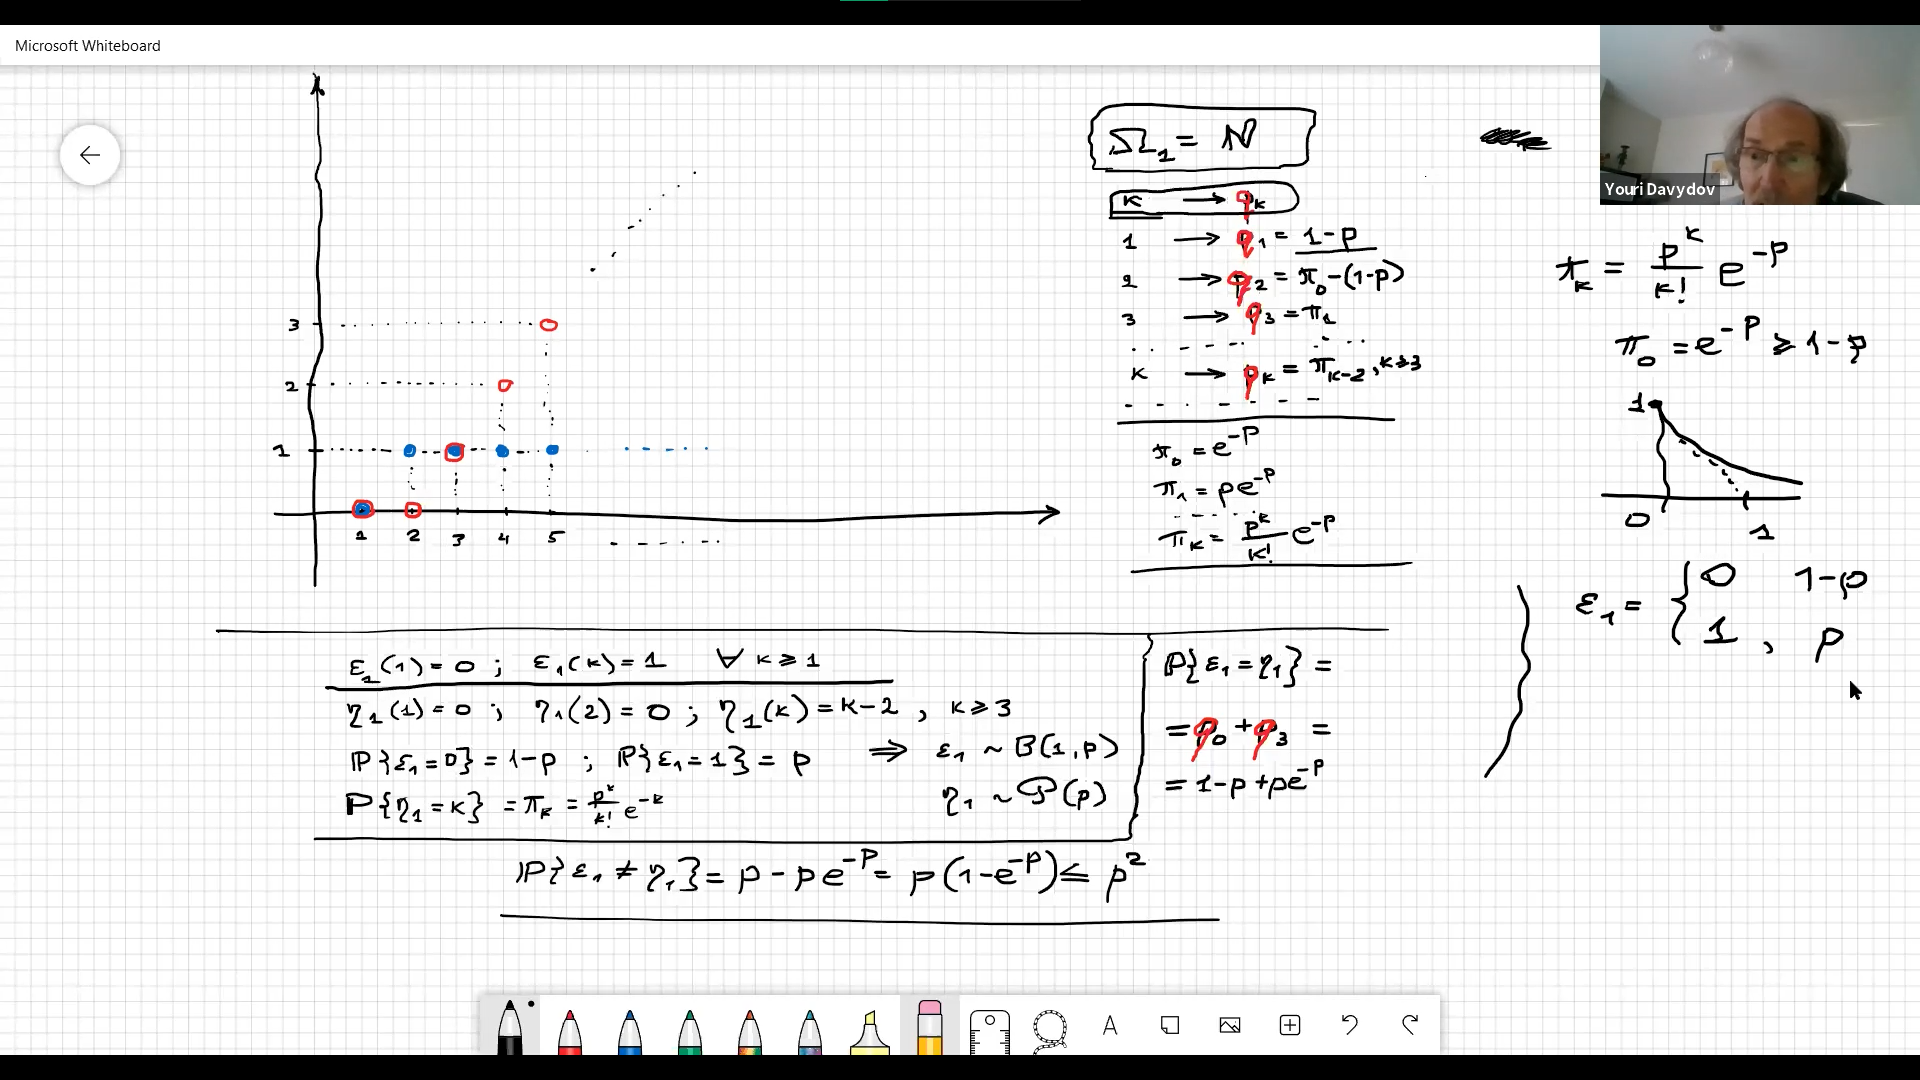
\includegraphics[width=\textwidth]{DPT-1.png}
            % \caption{Замена ручек лентами Мёбиуса}
            % \label{surface_typisation_picture_6}
            \todo[inline]{Перерисовать.}
        \end{figure}
        Несложно видеть, что
        \[\varepsilon_1 \Deq B(1, p), \qquad \text{ а } \qquad \eta_1 \Deq \mathcal{P}(p).\]
        При этом
        \[
            \PP_1\{\varepsilon_1 \neq \eta_1\}
            = 1 - \PP_1\{\varepsilon_1 = \eta_1\}
            = 1 - \PP_1(\{-1; 1\})
            = 1 - ((1-p) + p e^{-p})
            = p (1 - e^{-p})
            \leqslant p^2.
        \]

        Теперь сделаем ещё $n-1$ дубликатов нашего пространства и построенных случайных величин и перемножим их как в теореме \ref{probability-spaces-multiplication-theorem}. Получим пространство $(\Omega, \mathcal{F}, \PP)$ в котором выбраны случайные величины $\{\varepsilon_i\}_{i=1}^n$ и $\{\eta_i\}_{i=1}^n$, где
        \[\varepsilon_i \Deq B(1, n), \qquad \text{ а } \qquad \eta_i \Deq \mathcal{P}(p).\]
        При этом семейства $\{\varepsilon_i\}_{i=1}^n$ и $\{\eta_i\}_{i=1}^n$ независимы. Значит
        \[
            S_n \Deq B(n, p) \Deq X := \sum_{i=1}^n \varepsilon_i
            \qquad \text{ и } \qquad
            S \Deq \mathcal{P}(np) \Deq Y := \sum_{i=1}^n \eta_i.
        \]

        Следовательно
        \[
            \{X \neq Y\} \subseteq \bigcup_{i=1}^n \{\varepsilon_i \neq \eta_i\}
            \quad \Longrightarrow \quad
            \PP\{X \neq Y\} \leqslant \sum_{i=1}^n \PP\{\varepsilon_i \neq \eta_i\} \leqslant np^2.
        \]
        Отсюда имеем, что
        \begin{align*}
            |\PP\{S_n \in A\} - \PP\{S \in A\}|
            &= |\PP\{X \in A\} - \PP\{Y \in A\}|\\
            &= |\PP\{X \in A \wedge Y \notin A\} - \PP\{Y \in A \wedge X \notin A\}|\\
            &\leqslant \PP\{X \in A \wedge Y \notin A\} + \PP\{Y \in A \wedge X \notin A\}\\
            &\leqslant \PP\{X \neq Y\}\\
            &\leqslant np^2.
        \end{align*}
    \end{proof}

    \begin{corollary}
        Пусть дано $n \in \NN \cup \{0\}$ и случайные события $S_n \Deq B(n, p)$ и $S \Deq \mathcal{P}(np)$. Тогда
        \[\sum_{k=0}^\infty |\PP\{S_n = k\} - \PP\{S = k\}| \leqslant 2np^2.\] 
    \end{corollary}

    \begin{proof}
        Обозначим
        \[
            B_+ := \{k \mid \PP\{S_n = k\} \geqslant \PP\{S = k\}\}
            \qquad \text{ и } \qquad
            B_- := (\NN \cup \{0\}) \setminus B_+.
        \]
        Тогда понятно, что
        \begin{align*}
            \sum_{k=0}^\infty |\PP\{S_n = k\} - \PP\{S = k\}|
            &= \sum_{k \in B_+} (\PP\{S_n = k\} - \PP\{S = k\}) - \sum_{k \in B_-} (\PP\{S_n = k\} - \PP\{S = k\})\\
            &= (\PP\{S_n \in B_+\} - \PP\{S \in B_+\}) - (\PP\{S_n \in B_-\} - \PP\{S \in B_-\})\\
            &\leqslant |\PP\{S_n \in B_+\} - \PP\{S \in B_+\}| + |\PP\{S_n \in B_-\} - \PP\{S \in B_-\}|\\
            &\leqslant np^2 + np^2 = 2np^2
        \end{align*}
    \end{proof}

    \section{Математическое ожидание}

    \begin{definition}[для дискретной случайной величины]\label{discrete-expected-value-definition}
        Пусть даны вероятностное пространство $(\Omega, \mathcal{F}, \PP)$ и дискретная случайная величина $X$ в нём на $\RR$ (т.е. $X: \Omega \to \RR$ --- измеримая функция, что $X(\Omega)$ не более чем счётно). Тогда математическим ожиданием величины $X$ называется сумма
        \[\sum_{a \in X(\Omega)} a \PP\{X = a\},\]
        если она абсолютно сходится. Обозначение: $M(X)$ или $\EE(X)$.
    \end{definition}

    \begin{definition}[через интеграл Лебега]\label{Lebesgue-expected-value-definition}
        Пусть даны вероятностное пространство $(\Omega, \mathcal{F}, \PP)$ и случайная величина $X$ в нём на $\RR$ (т.е. $X: \Omega \to \RR$ --- измеримая функция). Тогда математическим ожиданием величины $X$ называется интеграл Лебега
        \[\int_\Omega X(\omega) \PP(d \omega),\]
        если он сходится. Обозначение: $M(X)$ или $\EE(X)$.
    \end{definition}

    \begin{statement}
        Определения \ref{discrete-expected-value-definition} и \ref{Lebesgue-expected-value-definition} равносильны в случаях, когда оба определены.
    \end{statement}

    \begin{remark}
        Несмотря на равносильность этих определений, мы пока не знаем интеграл Лебега. Поэтому будем определять математическое ожидание для дискретного случая. Но для непрерывного случая будем представлять, что математическое ожидание означает именно интеграл случайной величины по пространству.

        Также в случае дискретного пространства интеграл Лебега вырождается в сумму
        \[\sum_{\omega \in \Omega} X(\omega) \PP(\omega),\]
        что, понятно, равно определению для дискретной величины.
    \end{remark}

    \begin{lemma}\ 
        \begin{enumerate}
            \item $\EE(X)$ определено тогда и только тогда, когда $\EE(|X|)$ определено.
            \item \textbf{Линейность.} Для всяких случайных величин $X$ и $Y$ и констант $a$ и $b$ верно, что
                \[\EE(aX + bY) = a \EE(X) + b \EE(Y).\]
            \item \textbf{Положительность.} Если $X \geqslant 0$, то $\EE(X) \geqslant 0$.
            \item Если $X \leqslant Y$, то $\EE(X) \leqslant \EE(Y)$.
            \item $|\EE(X)| \leqslant \EE(|X|)$.
            \item \textbf{Неравенство Йенсена.} Пусть $\varphi: \RR \to \RR$ --- выпуклая функция. Тогда $\EE(\varphi(X)) \geqslant \varphi(\EE(X))$.
            \item Если $X$ и $Y$ имеют одинаковые распределения, то $\EE(X) = \EE(Y)$.
        \end{enumerate}
    \end{lemma}

    \begin{theorem}
        Пусть даны независимые случайные величины $X$ и $Y$ со сходящимися мат. ожиданиями. Тогда
        \[\EE(X \cdot Y) = \EE(X) \cdot \EE(Y).\]
    \end{theorem}

    \begin{proof}
        \begin{align*}
            \EE(X \cdot Y)
            &= \sum_{\substack{x \in X(\Omega)\\ y \in Y(\Omega)}} (x \cdot y) \PP\{X = x \wedge Y = y\}\\
            &= \sum_{\substack{x \in X(\Omega)\\ y \in Y(\Omega)}} x \cdot y \cdot \PP\{X = x\} \cdot \PP\{Y = y\}\\
            &= \left(\sum_{x \in X(\Omega)} x \cdot \PP\{X = x\}\right) \left(\sum_{y \in Y(\Omega)} y \cdot \PP\{Y = y\}\right)\\
            &= \EE(X) \cdot \EE(Y)\\
        \end{align*}
        Поскольку последние суммы --- мат. ожидания $X$ и $Y$ --- сходятся, то сходятся абсолютно, а значит абсолютно сходится и ряд-произведение. Значит мат. ожидание $X \cdot Y$ определено. 
    \end{proof}

    \begin{example}\ 
        \begin{enumerate}
            \item Пусть случайная величина $X \Deq B(n, p)$. Тогда по определению
                \[\EE(X) = \sum_{k=0}^n k \binom{n}{k} p^k (1-p)^{n-k},\]
                что считать непросто. С другой стороны пусть $\{\varepsilon_i\}_{i=1}^n$ --- независимые случайные величины с распределением $B(1, p)$. Тогда
                \[\EE(X) = \EE\left(\sum_{i=1}^n \varepsilon_i\right) = \sum_{i=1}^n \EE(\varepsilon_i) = np.\]
            \item Пусть случайная величина $X \Deq \mathcal{P}(\alpha)$. Тогда
                \[\EE(X) = \sum_{n=0}^\infty n \frac{\alpha^n}{n!} e^{-\alpha} = \alpha \sum_{n=0}^\infty \frac{\alpha^n}{n!} e^{-\alpha} = \alpha.\]
        \end{enumerate}
    \end{example}

    \begin{theorem}[неравенство Маркова]
        Пусть даны случайное событие $X \geqslant 0$ и некоторое значение $t > 0$. Тогда
        \[\PP\{X \geqslant t\} \leqslant \frac{\EE(X)}{t}.\]
    \end{theorem}

    \begin{proof}
        Рассмотрим множество (событие)
        \[A := \{\omega \in \Omega \mid X(\omega) \geqslant t\}\]
        Заметим, что
        \[t \ind_A \leqslant X,\]
        а значит
        \[\EE(X) \geqslant \EE(t \ind_A) = t \EE(\ind_A) = t \PP\{X \geqslant t\}.\]
    \end{proof}

    \begin{corollary}\label{Markov-inequality-theorem-functional-corollary}
        Пусть даны случайное событие $X$, произвольное подмножество $S \subseteq \RR$, что $X(\Omega) \subseteq S$, неотрицательно определённая неубывающая функция $f: S \to \RR$ и некоторая величина $t \in S$, что $f(t) > 0$. Тогда
        \[\PP\{X \geqslant t\} \leqslant \frac{\EE(f(X))}{f(t)}\]
    \end{corollary}

    \begin{proof}
        Заметим, что из неубываемости $f$ следует, что
        \[X \geqslant t \quad \Longrightarrow \quad f(X) \geqslant f(t),\]
        следовательно
        \[\PP\{X \geqslant t\} \leqslant \PP\{f(X) \geqslant f(t)\}.\]
        Применяя неравенство Маркова к $f(X)$ и $f(t)$ получаем
        \[\PP\{X \geqslant t\} \leqslant \PP\{f(X) \geqslant f(t)\} \leqslant \frac{\EE(f(X))}{f(t)}.\]
    \end{proof}

    \begin{example}
        \begin{enumerate}
            \item Пусть $f(x) = x^2$. Тогда применяя теорему к $|X|$ и $t > 0$, получаем, что
                \[\PP\{|x| \geqslant t\} \leqslant \frac{\EE(X^2)}{t^2}.\]
            \item Пусть $f(x) = e^{ax}$. Тогда применяя теорему к $X$ и $t$, получаем, что
                \[\PP\{X \geqslant t\} \leqslant \frac{\EE(e^{aX})}{e^{at}}.\]
        \end{enumerate}
    \end{example}

    \subsection{Дисперсия}

    \begin{definition}
        \emph{Дисперсия} случайной величины $X$ --- значение
        \[\EE\Bigl((X-\EE(X))^2\Bigr).\]
        Обозначение: $D(X)$ (в русской литературе), $\Var(X)$ (в английской литературе).
    \end{definition}

    \begin{lemma}\ 
        \begin{enumerate}
            \item $D(X)$ сходится тогда и только тогда, когда сходятся $E(X)$ и $E(X^2)$.
            \item $D(X) \geqslant 0$.
            \item $D(X) = 0 \Leftrightarrow \PP\{X \neq \EE(X)\} = 0$.
            \item $D(X + a) = D(X)$.
            \item $D(\lambda X) = \lambda^2 D(X)$.
            \item $D(X) = E(X^2) - E(X)^2$.
            \item Если $X$ и $Y$ независимы, то $D(X + Y) = D(X) + D(Y)$.
        \end{enumerate}
    \end{lemma}

    \begin{example}\ 
        \begin{enumerate}
            \item Пусть случайная величина $X \Deq B(n, p)$. Тогда по определению
                \[D(X) = \sum_{k=0}^n (k-np)^2 \binom{n}{k} p^k (1-p)^{n-k},\]
                что считать непросто. С другой стороны пусть $\{\varepsilon_i\}_{i=1}^n$ --- независимые случайные величины с распределением $B(1, p)$. Тогда
                \[
                    D(\varepsilon_i)
                    = \EE(\varepsilon_i^2) - \EE(\varepsilon_i)^2
                    = \EE(\varepsilon_i) - \EE(\varepsilon_i)^2
                    = p - p^2
                    = p(1-p)
                \]
                \[
                    D(X)
                    = D\left(\sum_{i=1}^n \varepsilon_i\right)
                    = \sum_{i=1}^n D(\varepsilon_i)
                    = np(1-p).
                \]
            \item Пусть случайная величина $X \Deq \mathcal{P}(\alpha)$. Тогда
                \[\EE(X(X-1)) = \sum_{n=0}^\infty n(n-1) \frac{\alpha^n}{n!} e^{-\alpha} = \alpha^2 \sum_{n=0}^\infty \frac{\alpha^n}{n!} e^{-\alpha} = \alpha^2,\]
                и следовательно
                \[D(X) = \EE(X(X-1)) + \EE(X) - \EE(X)^2 = \alpha^2 + \alpha - \alpha^2 = \alpha.\]
        \end{enumerate}
    \end{example}

    \begin{theorem}
        Пусть даны случайная величина $X$ и некоторая константа $t > 0$. Тогда
        \[\PP\{|X - \EE(X)| \geqslant t\} \leqslant \frac{D(X)}{t^2}.\]
    \end{theorem}

    \begin{proof}
        Применяя следствие \ref{Markov-inequality-theorem-functional-corollary} к $f(x) = x^2$, $Y := |X - \EE(X)|$ и $t > 0$, получаем
        \[\PP\{|X - \EE(X)| \geqslant t\} = \PP\{Y \geqslant t\} \leqslant \frac{\EE(Y^2)}{t^2} = \frac{D(X)}{t^2}.\]
    \end{proof}

    \subsection{Момент и ковариация}

    \begin{definition}
        Пусть $X$ --- случайная величина.
        \begin{itemize}
            \item $\EE(X^n)$ ($n \in \NN$) --- \emph{момент порядка $n$}.
            \item $\EE(|X|^\alpha)$ ($\alpha \in \RR$) --- \emph{абсолютный момент порядка $\alpha$}.
            \item $\EE((X - \EE(X))^n)$ ($n \in \NN$) --- \emph{центральный момент порядка $n$}.
            \item $\EE(|X - \EE(X)|^\alpha)$ ($\alpha \in \RR$) --- \emph{абсолютный центральный момент порядка $\alpha$}.
        \end{itemize}
    \end{definition}

    \begin{example}
        Дисперсия --- (абсолютный) центральный момент второго порядка.
    \end{example}

    \begin{definition}
        Пусть $X$, $Y$ --- случайные величины.
        \begin{itemize}
            \item $\EE(X^n Y^m)$ --- \emph{смешанный момент порядка $(n, m)$}.
            \item $\cov(X, Y) := \EE((X - \EE(X))(Y - \EE(Y)))$ --- \emph{ковариация}.
            \item $\rho(X, y) := \frac{\cov(X, Y)}{\sqrt{D(X) \cdot D(Y)}}$ --- \emph{коэффициент корреляции}, мера линейной зависимости.
        \end{itemize}
    \end{definition}

    \subsection{Закон больших чисел (ЗБЧ)}
    
    \begin{definition}
        Пусть даны последовательность случайных величин $(X_n)_{n=0}^\infty$ и случайная величина $X$. Тогда говорится, что $(X_n)_{n=0}^\infty$ \emph{сходится по вероятности} к $X$ и обозначается
        \[X_n \probto a \quad \text{ при } \quad n \to \infty,\]
    \end{definition}

    \begin{theorem}[ЗБЧ]
        Пусть дана последовательность независимых одинаково распределённых величин $(X_n)_{n=0}^\infty$, что $\EE(X_k) = a$, $D(X_k) = \sigma^2$. Пусть также $S_n := \sum_{k=0}^n X_k$. Тогда для всякого $\varepsilon > 0$
        \[\lim_{n \to \infty} \PP\left\{\left|\frac{S_n}{n} - a\right| \geqslant \varepsilon\right\} = 0,\]
        т.е.
        \[\frac{S_n}{n} \probto a \quad \text{ при } \quad n \to \infty.\]
    \end{theorem}

    \begin{proof}
        По неравенству Чебышёва
        \[
            \PP\left\{\left|\frac{S_n}{n} - a\right| \geqslant \varepsilon\right\}
            \leqslant \frac{D(S_n/n)}{\varepsilon^2}
            = \frac{1}{\varepsilon^2} \cdot \frac{1}{n^2} \cdot D(S_n)
            = \frac{1}{\varepsilon^2} \cdot \frac{1}{n^2} \cdot \sigma^2
            = \frac{\sigma^2}{\varepsilon^2} \cdot \frac{1}{n^2}
            \to 0
        \]
    \end{proof}

    \begin{theorem}[Хинчина]
        Пусть дана последовательность независимых одинаково распределённых величин $(X_n)_{n=0}^\infty$, что $\EE(X_k) = a$. Пусть также $S_n := \sum_{k=0}^n X_k$. Тогда
        \[\frac{S_n}{n} \probto a.\]
    \end{theorem}

    \begin{theorem}[Колмогорова]
        Пусть дана последовательность независимых одинаково распределённых величин $(X_n)_{n=0}^\infty$. Пусть также $S_n := \sum_{k=0}^n X_k$.
        \begin{enumerate}
            \item Пусть известно, что $\EE(X_k) = a$. Тогда $\frac{S_n}{n} \probto a$.
            \item Пусть известно, что $\frac{S_n}{n} \probto a$. Тогда $\EE(X_k) = a$.
        \end{enumerate}
    \end{theorem}

    \subsection{Практика}

    \begin{theorem}[\href{https://ru.wikipedia.org/wiki/\%D0\%A2\%D0\%B5\%D0\%BE\%D1\%80\%D0\%B5\%D0\%BC\%D0\%B0\_\%D0\%92\%D0\%B5\%D0\%B9\%D0\%B5\%D1\%80\%D1\%88\%D1\%82\%D1\%80\%D0\%B0\%D1\%81\%D1\%81\%D0\%B0\_\%E2\%80\%94\_\%D0\%A1\%D1\%82\%D0\%BE\%D1\%83\%D0\%BD\%D0\%B0\#\%D0\%A2\%D0\%B5\%D0\%BE\%D1\%80\%D0\%B5\%D0\%BC\%D0\%B0\_\%D0\%92\%D0\%B5\%D0\%B9\%D0\%B5\%D1\%80\%D1\%88\%D1\%82\%D1\%80\%D0\%B0\%D1\%81\%D1\%81\%D0\%B0}{аппроксимационная теорема Вейерштрасса}]
        Пусть дана непрерывная функция $f: [0; 1] \to \RR$. Тогда для всякого $\varepsilon > 0$ есть многочлен $Q \in \RR[x]$, что $|f - Q| < \varepsilon$ на отрезке $[0; 1]$.

        Говоря иначе, есть последовательность многочленов $(Q_n)_{n=0}^\infty$ из $\RR[x]$, что
        \[\lim_{n \to \infty} \sup_{[0; 1]} |f - Q_n| = 0.\]
    \end{theorem}

    \begin{proof}[Доказательство Бернштейна]
        Рассмотрим последовательность независимых случайных величин $(\xi_k)_{k=1}^\infty$ с распределением $B(1, p)$. Также обозначим $S_n := \sum_{k=1}^n \xi_k$. Поскольку $S_n \Deq B(n, p)$, то рассмотрим
        \[Q_n(p) := \EE f\left(\frac{S_n}{n}\right) = \sum_{k=0}^n f\left(\frac{k}{n}\right) P_{n,k}(p) = \sum_{k=0}^n f\left(\frac{k}{n}\right) \binom{n}{k} p^k (1-p)^{n-k}\]
        --- многочлен от $p$, где
        \[P_{n, k}(p) := \binom{n}{k} p^k (1-p)^{n-k}.\]
        Тогда
        \[
            \Delta_n(p)
            = |Q_n(p) - f(p)|
            = \left|\EE f\left(\frac{S_n}{n}\right) - \EE f(p)\right|
            = \left|\EE \left(f\left(\frac{S_n}{n}\right) - f(p)\right)\right|
            \leqslant \EE \left|f\left(\frac{S_n}{n}\right) - f(p)\right|.
        \]

        Обозначим за
        \[\omega_f(h) := \sup_{\substack{t, s \in [0; 1]\\ |t-s| \leqslant h}} |f(t) - f(s)|.\]
        Зафиксируем какое-нибудь $\delta > 0$. Заметим, что
        \[
            \EE \left|f\left(\frac{S_n}{n}\right) - f(p)\right| =
            \underbrace{\sum_{k:\; \left|\frac{k}{n} - p\right| \leqslant \delta} \left|f\left(\frac{S_n}{n}\right) - f(p)\right| P_{n, k}(p)}_{\Sigma_1} +
            \underbrace{\sum_{k:\; \left|\frac{k}{n} - p\right| > \delta} \left|f\left(\frac{S_n}{n}\right) - f(p)\right| P_{n, k}(p)}_{\Sigma_2}.
        \]
        Тогда
        \[
            \Sigma_1
            \leqslant \sum_{k:\; \left|\frac{k}{n} - p\right| \leqslant \delta} \omega_f(\delta) \cdot P_{n, k}(p)
            \leqslant \omega_f(\delta).
        \]
        Пусть также $M := \osc_{[0; 1]} f$, тогда
        \[
            \Sigma_2
            \leqslant M \sum_{k:\; \left|\frac{k}{n} - p\right| > \delta} P_{n, k}(p)
            = M \PP\left\{\left|\frac{S_n}{n}-p\right| > \delta\right\}
            \leqslant M \frac{D\left(\frac{S_n}{n}\right)}{\delta^2}
            = \frac{Mp(1-p)}{\delta^2 n}
            \leqslant \frac{M}{4\delta^2} \cdot \frac{1}{n}.
        \]
        Таким образом
        \[\Delta_n(p) \leqslant \omega_f(\delta) + \frac{M}{4\delta^2} \cdot \frac{1}{n}.\]
        По равномерной непрерывности $f$ для всякого $\varepsilon > 0$ есть $\delta > 0$, что $\omega_f(\delta) < \varepsilon/2$. А тогда есть и $N \in \NN$, что для всякого $n \geqslant N$
        \[\frac{M}{4\delta^2} \cdot \frac{1}{n} < \frac{\varepsilon}{2},\]
        т.е. для всех $n \in \NN$
        \[|Q_n(p) - f(p)| < \varepsilon.\]
        А значит
        \[\lim_{n \to \infty} \sup_{[0; 1]} |f - Q_n| = 0.\]
    \end{proof}

    \todo[inline]{Написать про нормальные числа (или нет смысла?). См. лекцию №5 от 16.03, примерно с 40:05.}

    \section{Случайные блуждания (?)}

    \subsection{Простое одномерное блуждание}

    Пусть мы находимся на $\ZZ$ и каждый момент двигаемся либо с вероятностью $1/2$ на $+1$, либо с вероятностью $1/2$ на $-1$. В таком случае, можно считать, что наше вероятностное пространство задаётся как
    \begin{itemize}
        \item $\Omega := \{1; -1\}^\NN$ --- множество счётных последовательностей с элементами из $\{1; -1\}$,
        \item $\mathcal{F}$ --- минимальная сигма-алгебра, содержащая все $A_{n, s}$,
        \item $\PP$ задаётся так, что $\PP(A_{n,s}) = 1/2$ для всех $n \in \NN$, $s \in \{1; -1\}$,
    \end{itemize}
    где $A_{n,s}$ подмножество всех последовательностей, у которых на месте $n$ стоит $s$ ($n \in \NN$, $s \in \{1; -1\}$). (Почему $\PP$ существует и единственно, опустим.)

    Также рассмотрим случайные величины
    \[
        \varepsilon_k :=
        \begin{cases}
            1& \text{ если } \omega \in A_{k,1},\\
            -1& \text{ если } \omega \in A_{k,-1}.
        \end{cases}
    \]
    (изменения координаты на шаге $k$) и
    \[S_n := \sum_{k=1}^n \varepsilon_k\]
    координата после шага $n$.

    \begin{lemma}
        \[
            \PP\{S_n = k\} =
            \begin{cases}
                0& \text{ если } n \not\equiv k \mod{2},\\
                \binom{n}{\frac{n+k}{2}}& \text{ иначе}.
            \end{cases}
        \]
    \end{lemma}

    \begin{theorem}
        Пусть играют два игрока. В начале у первого имеется капитал в размере $a$, а у второго --- $b$ ($a, b \in \NN \cup \{0\}$). Каждый ход подбрасывается монетка; при выпадении орла первый даёт единицу капитала второму, а при выпадении решки --- наоборот.
        \begin{enumerate}
            \item Вероятность разорения первого равна $\frac{b}{a+b}$.
            \item Вероятность разорения кого-нибудь равна $1$.
        \end{enumerate}
    \end{theorem}

    \begin{proof}
        Будем в каждый момент времени откладывать на целочисленный оси капитал первого. Тогда начинаем мы в $a$, каждый ход случайно сдвигаемся либо с вероятностью $1/2$ на $+1$, либо с вероятностью $1/2$ на $-1$, а заканчиваем игру, если попали в $0$ (первый обанкротился), либо в $a + b$ (второй обанкротился).

        Заметим, что вероятность разорения первого при фиксированном $a+b$ есть функция от $a$ --- $f(a)$. Понятно, что
        \[f(0) = 1, \qquad f(a + b) = 0.\]
        При этом если $a \in (0; a + b)$, то с вероятностью $1/2$ он спустится в $a-1$, откуда вероятность обанкротится станет равна $f(a-1)$, а с вероятностью $1/2$ --- поднимется и вероятность станет равна $f(a+1)$. Следовательно
        \[f(a) = \frac{1}{2} f(a-1) + \frac{1}{2} f(a).\]
        Таким образом
        \[f(a) = Ka + L;\]
        подставляя точки $0$ и $a+b$, получаем
        \[f(a) = \frac{b}{a+b}.\]

        По аналогии вероятность того, что второй обанкротится равна $\frac{a}{a+b}$. Поэтому вероятноость того, что уто-то обанкротится равна $1$.
    \end{proof}

    \begin{theorem}[следствие теоремы Пойа]
        Вероятность вернуться в $0$ равна $1$.
    \end{theorem}

    \begin{proof}
        Рассмотрим вероятности
        \[
            p_n := \PP\{S_n = 0\} = \PP\{\text{``вернуться в $0$ за $n$ шагов''}\}, \qquad p_0 = 1
        \]
        и
        \[0
            f_n := \PP\left\{S_n = 0 \wedge \bigwedge_{k=1}^{n-1}\right\} = \PP\{\text{``вернуться в $0$ ровно за $n$ шагов''}\}, \qquad f_0 = 1.
        \]
        Понятно, что вероятность вернуться в $0$ когда-нибудь равна
        \[\sum_{n=1}^\infty f_n.\]
        
        Заметим, что для всякого $n \geqslant 1$ вероятность вернуться в $0$ за $n$ шагов можно разбить по случаям первого возвращения в $0$ (от $1$ до $n$), а значит
        \[p_n = \sum_{k=1}^{n} f_k p_{n-k}.\]
        При этом поскольку мы взяли $f_0 = 0$, то
        \[p_n = \sum_{k=0}^n f_k p_{n-k}.\]

        Пусть $F$ и $P$ --- производящие функции $\{f_n\}_{n=0}^\infty$ и $\{p_n\}_{n=0}^\infty$. Тогда из предыдущего равенства мы получаем, что
        \[P(t) - 1 = F(t) P(t),\]
        т.е.
        \[P(t) = \frac{1}{1 - F(t)}.\]
        Заметим, что $F$ и $G$ сходятся в $1$-окрестности нуля, $F$ сходится в $1$, и мы ищем значение $F(1)$. Поэтому несложно понять, что $F(1) = 1$ тогда и только тогда, когда $G(1) = \infty$.

        При этом несложно понять, что
        \[
            p_{2n+1} = 0, \qquad p_{2n} = \frac{1}{2^{2n}}\binom{2n}{n} \approx \frac{1}{\sqrt{\pi n}},
        \]
        значит $G(1) = \infty$.
    \end{proof}

    \subsection{Непростое одномерное блуждание}

    Теперь зафиксируем $p \in [0; 1]$ и рассмотрим похожее вероятностное пространство: $\Omega$ и $\mathcal{F}$ такие же, а $\PP$ определено так, что
    \[
        \PP(A_{n,s}) =
        \begin{cases}
            p& \text{ если } s = 1,\\
            1-p& \text{ если } s = -1.
        \end{cases}
    \]
    
    Несложно видеть, что по ЗБЧ
    \[\frac{S_n}{n} \probto \EE(\varepsilon_1) = p - (1-p) = 2p - 1,\]
    т.е. почти везде $S_n = (2p - 1) n (1 + o(1))$. Таким образом ``понятно'', что возвратность будет только при $p = 1/2$.

    \begin{theorem}
        В таком случае случайное блуждание невозвратно.
    \end{theorem}

    \begin{proof}
        Рассуждение с формальными рядами $F$ и $P$ не меняется. В таком случае
        \[p_{2n} = \binom{2n}{n} p^n (1-p)^n \approx \frac{(4p(1-p))^n}{\sqrt{\pi n}}.\]
        Но $4p(1-p) \leqslant 1$, а равенство достигается только для $p = 1/2$. Следовательно при $p \neq 1/2$ ряд $P(1)$ сходится, а тогда $F(1) < 1$, т.е. блуждание невозвратно.
    \end{proof}

    \begin{theorem}
        Если блуждание возвратно, то вероятность вернуться в $0$ бесконечно много раз равна $1$. Иначе эта же вероятность равна $0$.
    \end{theorem}

    \begin{proof}
        Пусть $R_n$ --- событие возвращения $n$ раз, а $r_n := \PP(R_n)$. Понятно, что $R_{n + 1} \subseteq R_n$.
        \[r_{n+1} = \PP(R_{n+1}) = \PP(R_{n+1} \mid R_n) \PP(R_n) = \PP(R_1) \PP(R_n) = r_1 r_n = r_1^{n+1}.\]
        Значит вероятность возвращения бесконечное число раз равна
        \[
            \lim_{n \to \infty} \PP(R_n)
            = \lim_{n \to \infty} r_1^n
            = \begin{cases}
                1& \text{ если } r_1 = 1,\\
                0& \text{ если } r_1 < 1.
            \end{cases}
        \]
    \end{proof}

    \subsection{Простой одномерный случай}

    Теперь мы рассмотрим ещё одно вероятностное пространство. Зафиксируем размерность $d$, пространство $\RR^d$ и множество шагов $S := \{\pm e_k\}_{k=0}^d$. Тогда по аналогии определим $\Omega := S^\NN$, $A_{n, s}$ (для всех $n \in \NN$, $s \in S$), $\mathcal{F}$, $\PP$, $\varepsilon_n$ и $S_n$.

    \begin{theorem}[Пойа]
        Блуждание возвратно тогда и только тогда, когда $d \in \{1; 2\}$.
    \end{theorem}

    \begin{proof}[Основные наброски доказательства.]
        Рассуждение с рядами $P$ и $F$ остаются неизменными. Поэтому нужно понять, когда $P(1) = \infty$.

        В случае $d = 2$ имеем, что
        \[
            p_n
            = \sum_{k=0}^n \frac{\binom{2n}{k, k, n-k, n-k}}{4^{2n}}
            = \frac{\binom{2n}{n}}{4^{2n}} \sum_{k=0}^n \binom{n}{k}^2
            = \frac{\binom{2n}{n}^2}{4^{2n}}
            \approx \frac{1}{\sqrt{\pi n}^2},
        \]
        откуда сразу получается, что $P(1)$ рассходится.

        В общем случае можно показать, что
        \[p_n = O(n^{-\frac{d}{2}}),\]
        откуда так же сразу получается, что $P(1)$ сходится тогда и только тогда, когда $d > 2$.
    \end{proof}

    Также точно так же как в случае $d = 1$ можно показать, что если $f: \ZZ^d \to [0; 1]$ --- вероятность вернуться из $x$ в $0$, то для всякого $x \in \ZZ^d$ 
    \[f(x) = \frac{1}{2d} \sum_{s \in S} f(x + s).\]
    В таком случае можно показать, что $f = 1$. Отсюда сразу можно получить, что случайное блуждание из $0$ в каждую точку попадёт с вероятностью $1$ (вероятность для каждой точки по отдельности).

    \subsection{Закон арксинуса}

    Будем рассматривать простое одномерное блуждание. Обозначим
    \[
        T_+(n) := \sum_{k=1}^n \ind_{\{S_{k-1} \geqslant 0 \wedge S_k \geqslant 0\}}
        \qquad \text{ и } \qquad
        T_-(n) := \sum_{k=1}^n \ind_{\{S_{k-1} \leqslant 0 \wedge S_k \leqslant 0\}}
    \]
    --- ``время пребывания на $\RR_+$'' и ``время пребывания на $\RR_-$''. Понятно, что $T_+$ и $T_-$ одинаково распределены и зависимы (так как $T_+(n) + T_-(n) = n$).

    \begin{exercise}
        Для всякого $n \in \NN$
        \[T_+(2n)\]
        принимает только чётные значения.
    \end{exercise}

    \begin{lemma}[см. Ширяев, ``Вероятность'', гл. I, \textsection 10 (стр. 129, лемма 2 по изданию 2007 года)]\label{arcsine-law-theorem-lemma}
        \[\PP\{T_+(2n) = 2k\} = \PP\{S_{2k} = 0\} \cdot \PP\{S_{2(n-k)} = 0\}\]
    \end{lemma}

    \begin{theorem}[закон арксинуса]
        Для всяких $0 < a < b < 1$
        \[
            \lim_{n \to \infty} \PP\left\{\frac{T_+(2n)}{2n} \in [a; b]\right\}
            = \frac{1}{\pi} \int_a^b \frac{dt}{\sqrt{t(1-t)}}
            = \frac{2}{\pi} (\sin^{-1}(\sqrt{b}) - \sin^{-1}(\sqrt{a}))
        \]
    \end{theorem}

    \begin{proof}
        Из утверждения \ref{arcsine-law-theorem-lemma} понятно, что
        \[
            \PP\left\{\frac{T_+(2n)}{2n} \in [a; b]\right\}
            = \sum_{2na \leqslant 2k \leqslant 2nb} \PP\{T_+(2n) = 2k\}
        \]
        Следовательно все рассматриваемые $k \sim n$, а поэтому
        \[
            \PP\{T_+(2n) = 2k\}
            = \PP\{S_{2k} = 0\} \cdot \PP\{S_{2(n-k)} = 0\}
            = \frac{\binom{2k}{k}}{2^{2k}} \cdot \frac{\binom{2(n-k)}{n-k}}{2^{2(n-k)}}
            \approx \frac{1}{\pi \sqrt{k(n-k)}}
            = \frac{1}{\pi} \cdot \frac{1}{n} \cdot \frac{1}{\sqrt{\frac{k}{n}(1-\frac{k}{n})}}.
        \]
        Следовательно при $n \to \infty$
        \[
            \PP\left\{\frac{T_+(2n)}{2n} \in [a; b]\right\}
            \approx \frac{1}{\pi} \sum_{\frac{k}{n} \in [a; b]} \frac{1}{n} \cdot \frac{1}{\sqrt{\frac{k}{n}(1-\frac{k}{n})}},
        \]
        т.е. вырождается в интегральную сумму функции $\frac{1}{\pi} \cdot \frac{1}{t(1-t)}$ на отрезке $[a; b]$. Таким образом
        \[\lim_{n \to \infty} \PP\left\{\frac{T_+(2n)}{2n} \in [a; b]\right\} = \frac{1}{\pi} \int_a^b \frac{dt}{t(1-t)}.\]
    \end{proof}

    \subsection{Распределение максимума}

    Рассмотрим теперь случайную величину
    \[M_n := \max_{k = 0}^n S_k.\]
    
    Понятно, что $M_n \geqslant 0$. Также несложно заметить, что
    \begin{align*}
        \PP\{M_n \geqslant j\}
        &= \PP\{M_n \geqslant j \wedge S_n \geqslant j\} + \PP\{M_n \geqslant j \wedge S_n < j\}\\
        &= \PP\{S_n \geqslant j\} + \PP\{M_n \geqslant j \wedge S_n < j\}\\
        &= \PP\{S_n \geqslant j\} + \PP\{S_n > j\}\\
        &= 2\PP\{S_n \geqslant j\} - \PP\{S_n > j\}.
    \end{align*}
    (Так как если $S_n < j$, то путь после первого достигания $j$ можно отразить и получить биекцию со случаями $S_n > j$.)

    \subsection{Центральная предельная теорема (ЦПТ)}

    Теперь будем рассматривать испытания Бернулли c распределением $B(1, p)$, где $p \in (0; 1)$, и определённые в таком случае $\{\xi_n\}_{n=1}^\infty$ и $\{S_n\}_{n=0}^\infty$. Вспомним, что тогда
    \[\PP\{S_n = k\} = \binom{n}{k} p^k (1-p)^{n-k}.\]

    \begin{theorem}[локальная теорема Муавра-Лапласа]
        Для всякой последовательности $\{\varepsilon_n\}_{n=1} \to 0$
        \[\PP\{S_n = k\} = \frac{1}{\sqrt{2\pi n p (1-p)}} \cdot e^{-\frac{x_k^2}{2}} (1 + o(1))\]
        равномерно по всем $k \in [np - \varepsilon_n n^{2/3}; np + \varepsilon_n n^{2/3}]$, где
        \[x_k = \frac{k - np}{\sqrt{np(1-p)}}.\]
    \end{theorem}

    \begin{proof}
        Понятно, что $k = np(1 + o(1))$ и $n-k = n(1-p)(1 + o(1))$. Следовательно, применяя формулу Стирлинга,
        \begin{align*}
            \PP\{S_n = k\}
            &\approx \frac{1}{\sqrt{2\pi n}} \cdot \frac{1}{\sqrt{\frac{k}{n}(1-\frac{k}{n})}} \cdot \frac{n^n}{k^k(n-k)^{n-k}} \cdot p^k (1-p)^k\\
            &\approx \frac{1}{\sqrt{2\pi n p (1-p)}} \cdot \left(\frac{np}{k}\right)^k \cdot \left(\frac{n(1-p)}{n-k}\right)^{n-k}.
        \end{align*}
        Пусть $v := k - np = o(n^{2/3})$. Заметим, что
        \[
            \ln\left(\frac{np}{k}\right)^k
            = -k \ln\left(1 + \frac{v}{np}\right)
            = -(np + v)\left(\frac{v}{np} - \frac{v^2}{2(np)^2} + o\left(\frac{v^3}{(np)^3}\right)\right)
            = v + \frac{v^2}{2np} + o(1)
        \]
        Аналогично
        \[
            \ln\left(\frac{n(1-p)}{n-k}\right)^{n-k}
            = -v + \frac{v^2}{2n(1-p)} + o(1),
        \]
        откуда
        \[
            \ln\left(\left(\frac{np}{k}\right)^k \cdot \left(\frac{n(1-p)}{n-k}\right)^{n-k}\right)
            = -\frac{v^2}{2np(1-p)} + o(1)
            = -\frac{x_k^2}{2} + o(1).
        \]
        Следовательно
        \[\PP\{S_n = k\} \approx \frac{1}{\sqrt{2\pi n p (1-p)}} \cdot e^{-\frac{x_k^2}{2}}.\]

        Равномерность получается внимательным всматриванием в доказательство.
    \end{proof}

    \begin{theorem}[интегральная теорема Муавра-Лапласа]
        Пусть
        \[Z_n := \frac{S_n - np}{\sqrt{np(1-p)}}.\]
        Тогда
        \[\lim_{n \to \infty} \PP\{Z_n \in [a; b]\} = \frac{1}{\sqrt{2\pi}} \int_a^b e^{-\frac{x^2}{2}} dx\]
        и сходимость равномерна по $a$ и $b$.
    \end{theorem}

    \begin{proof}
        По локальной теореме Муавра-Лапласа имеем, что
        \[
            \PP\{Z_n \in [a; b]\}
            = \sum_{k: \frac{k - np}{\sqrt{np(1-p)}}} \PP\{S_n = k\}
            = \frac{1}{2\pi} \cdot \frac{1}{\sqrt{np(1-p)}} \sum_{k: \frac{k - np}{\sqrt{np(1-p)}}} e^{-\frac{x_k^2}{2}} (1 + r_{n, k}),
        \]
        где $r_{n, k} = o(1)$ равномерно на всём рассматриваемом отрезке. Следовательно
        \[
            \lim_{n \to \infty} \PP\{Z_n \in [a; b]\}
            = \frac{1}{2\pi} \cdot \lim_{n \to \infty} \frac{1}{\sqrt{np(1-p)}} \sum_{k: \frac{k - np}{\sqrt{np(1-p)}}} e^{-\frac{x_k^2}{2}}
            = \frac{1}{2\pi} \int_a^b e^{-\frac{x^2}{2}} dx.
        \]
        
        Равномерность получается из того, что
        \[\varphi_n(b) := \PP\{Z_n \in [-\infty; b]\} \qquad \text{ и } \qquad \varphi_n(b) := \frac{1}{2\pi} \int_a^b e^{-\frac{x^2}{2}} dx\]
        --- монотонно неубывающие ограниченные (так как лежат в $[0; 1]$) функции на $\RR$, и имеется поточечная сходимость $\{\varphi_n\}_{n=0}^\infty \to \varphi$; поэтому должна быть и равномерная сходимость, а следовательно и равномерная сходимость $\varphi_n(b) - \varphi_n(a)$.
    \end{proof}

    \begin{theorem}[Paul Lévy, анонс]
        Пусть $\{X_n\}_{n=0}^\infty$ --- независимые одинаково распределённые случайные величины, что $\EE(X_n) = A$ и $D(X_n) = \sigma^2$ ($\sigma^2 < \infty$). Пусть также
        \[S_n = \sum_{k=1}^n X_k.\]
        Тогда
        \[\lim_{n \to \infty} \PP\left\{\frac{S_n - \EE(S_n)}{\sqrt{D(S_n)}} \in [a; b]\right\} = \frac{1}{\sqrt{2\pi}} \int_a^b e^{-\frac{x^2}{2}}dx\]
        и сходимость равномерно по $a$ и $b$.
    \end{theorem}

    \begin{remark}
        Понятно, что эта теорема является значительным расширением интегральной теоремы Муавра-Лапласа.
    \end{remark}

    \subsection{Производящие функции}

    \begin{definition}
        Пусть дана случайная величина $X$ с множеством значений $X(\Omega) = \NN \cup \{0\}$. Обозначим $p_k := \PP\{X = k\}$. Тогда \emph{производящей функцией $X$} называется функция (или ряд)
        \[\varphi_X(z) = \EE(z^X) = \sum_{k=0}^\infty p_k z^k.\]
    \end{definition}

    \begin{lemma}\ 
        \begin{enumerate}
            \item $\varphi$ определена в $U_1(0)$.
            \item $\varphi_X(t)$ выпукла на $[0; 1]$.
            \item $\frac{\varphi_X^{(n)}(0)}{n!} = \PP\{X = n\}$.
            \item $\varphi_X(1) = 1$.
            \item Для независимых $X$ и $Y$ верно, что $\varphi_{X + Y} = \varphi_X \varphi_Y$.
            \item \textbf{Связь с моментами.} Если $\EE(X^n) < \infty$, то
                \[\varphi_X^{(n)}(1) = \EE\left(\prod_{k=0}^{n-1} X - k\right).\]
        \end{enumerate}
    \end{lemma}

    \subsubsection{Сумма случайного числа случайных величин}

    \begin{theorem}
        Пусть даны набор независимых случайных величин $\{X_n\}_{n=1}^\infty$ с множеством значений $\NN \cup \{0\}$ и распределением вероятностей $\PP\{X_i = k\} = p_k$, их производящая функция $\varphi$, независящая от них случайная величина $\tau$ с множеством значений $\NN \cup \{0\}$. Обозначим
        \[S_n := \sum_{k=1}^n X_k \qquad \text{ и } \qquad U = S_\tau = \sum_{k=1}^\tau X_k.\]
        Тогда
        \[\varphi_U(z) = \varphi_\tau(\varphi(z)).\]
    \end{theorem}

    \begin{proof}
        \begin{align*}
            \varphi_U(z)
            &= \sum_{k=0}^\infty \PP\{U = k\} z^k&
            &= \sum_{k=0}^\infty \sum_{n=0}^\infty \PP\{U = k \wedge \tau = n\} z^k\\
            &= \sum_{n=0}^\infty \sum_{k=0}^\infty \PP\{\tau = n \wedge S_n = k\} z^k&
            &= \sum_{n=0}^\infty \PP\{\tau = n\} \sum_{k=0}^\infty \PP\{S_n = k\} z^k\\
            &= \sum_{n=0}^\infty \PP\{\tau = n\} \varphi_{S_n}(z)&
            &= \sum_{n=0}^\infty \PP\{\tau = n\} \varphi(z)^n\\
            &= \varphi_{\tau}(\varphi(z)).
        \end{align*}
    \end{proof}

    \section{Цепи Маркова}

    \subsection{Ветвящиеся процессы}

    \begin{definition}[ветвящийся процесс Гальтона-Ватсона]
        Пусть фиксирован набор вероятностей $\{p_n\}_{n=0}^\infty$, что $\sum_{n=0}^\infty p_n = 1$. Рассмотрим вероятностное пространство, в котором
        \begin{itemize}
            \item $\Omega := \NN^{\NN \times \NN}$ --- множество двумерных последовательностей с натуральными индексами с элементами из $\NN$,
            \item $\mathcal{F}$ --- минимальная сигма-алгебра, содержащая все $A_{n, m, c}$,
            \item $\PP$ задаётся так, что $\PP(A_{n, m, c}) = p_c$ для всех $n \in \NN$, $s \in \{1; -1\}$,
        \end{itemize}
        где $A_{n, m, c}$ --- множество последовательностей, у которых на месте $(n, m)$ стоит $c$. Рассмотрим случайные величины
        \[
            X_{n, m} =
            \begin{cases}
                c& \text{ если } \omega \in A_{n, m, c}\\
                \dots,
            \end{cases}
        \]
        и
        \[M_0 = 1, \qquad M_{n+1} = \sum_{k=1}^{M_n} X_{n, k}.\]
        Также обозначим $\varphi$ --- характеристическую функцию $X$.

        Это можно интерпретировать следующим образом. Пусть у нас есть частица. В первый момент она делится на некоторое количество таких же частиц, равное случайной величине $X_{0, 1}$. Во второй момент каждая $k$-ая частица делится на $X_{1, k}$ частиц; и так происходит далее. При этом все $X_{n, m}$ независимы и одинаково распределены. И таким образом $M_n$ будет количеством частиц после момента $n$.
    \end{definition}

    \begin{lemma}
        \[\varphi_n(z) := \varphi_{M_n}(z) = \varphi^n(z).\]
    \end{lemma}

    \begin{proof}
        $\varphi_0(z) = \varphi^0(z)$ и
        \[\varphi_{n+1}(z) = \varphi_{M_{n+1}}(z) = \varphi_{M_n}(\varphi(z)) = \varphi^n(z).\]
    \end{proof}

    \begin{definition}
        \[R_n := \{M_n = 0\} \qquad \text{ и } \qquad R := \bigcup_{n=0}^\infty R_n\]
        --- события вырождения процесса в момент $n$ и вырождения (когда-нибудь), а
        \[q_n := \PP(R_n) \qquad \text{ и } \qquad q := \PP(R)\]
        --- вероятности вырождения процесса в момент $n$ и вырождения (когда-нибудь).
    \end{definition}

    \begin{lemma}\ 
        \begin{enumerate}
            \item $R_n \subseteq R_{n+1}$.
            \item $q_n \leqslant q_{n+1}$.
            \item $q = \lim_{n \to \infty} q_n$.
        \end{enumerate}
    \end{lemma}

    \begin{theorem}
        $q$ является наименьшим корнем уравнения $\varphi(t) = t$ на $[0; 1]$.
    \end{theorem}

    \begin{proof}
        Для начала заметим, что $\varphi$ как функция $[0; 1] \to [0; 1]$ обладает следующими свойствами.
        \begin{enumerate}
            \item $\varphi(0) = p_0$ и $\varphi(1) = 1$.
            \item $\varphi$ монотонна
            \item $\varphi$ выпукла.
            \item $\varphi$ либо прямая, либо пересекает всякую прямую не более чем в двух точках.
            \item\ 
                \begin{enumerate}
                    \item Если $\varphi \geqslant t$ и равенство достигается только в $1$, то корнем будет только $1$.
                    \item Если $\varphi$ --- прямая, не подходящая под первый пункт, то уравнения $\varphi(t) = t$ множеством корней будет весь $[0; 1]$.
                    \item Если $\varphi$ --- не прямая, не подходящая под первый пункт, то у уравнения $\varphi(t) = t$ есть ровно один корень отличный от $1$.
                \end{enumerate}
            \item $\varphi(t) - t$ до первого корня положительна, а между корнями отрицательна.
        \end{enumerate}

        Теперь заметим, что
        \[q_0 = p_0 \qquad \text{ и } \qquad q_{n+1} = \varphi^{n+1}(0) = \varphi(q_n).\]
        Следовательно, поскольку $\varphi$ непрерывна на $[0; 1]$, переходя к пределу, получаем, что $\varphi(q) = q$. При этом так как $q_n \leqslant q_{n+1}$, то $\varphi(t) - t$ в точках $q_n$ положительно, откуда следует, что $q_n$ меньше наименьшего корня. Значит $q$ является наименьшим корнем.
    \end{proof}

    \begin{theorem}
        TFAE
        \begin{enumerate}
            \item $q < 1$.
            \item Либо $\EE(X) > 1$, либо $\PP\{X = 1\} = 1$.
        \end{enumerate}
    \end{theorem}

    \begin{proof}
        \begin{itemize}
            \item[$2 \Rightarrow 1)$] Если $\PP\{X = 1\} = 1$, то $\varphi(t) = t$. В таком случае $M_n = 1$ с вероятностью $1$, а тогда $q = 0 < 1$.

                Если же $\EE(X) > 1$, то $\varphi'(1) = \EE(X) > 1$, значит левее точки $1$ локально функция $\varphi(t) - t$ отрицательна, откуда $1$ --- не минимальный корень. Т.е. $q < 1$.
            
            \item[$1 \Rightarrow 2)$] Если $q < 1$, то либо $\varphi(t) = t$, т.е. $\PP{X = 1} = 1$, либо $\varphi(t) - t$ на промежутке $(q; 1)$ отрицательна и выпукла, т.е. $\varphi'(t)$ возрастает и следовательно $\varphi'(1) > 1$, откуда $\EE(X) = \varphi'(1) = 1$.
        \end{itemize}
    \end{proof}

    \begin{definition}
        Ветвящийся процесс называется
        \begin{itemize}
            \item \emph{надкритическим}, если $\EE(X) > 1$,
            \item \emph{критическим}, если $\EE(X) = 1$,
            \item \emph{подкритическим}, если $\EE(X) < 1$.
        \end{itemize}
    \end{definition}

    \subsection{Цепи Маркова}

    \begin{definition}
        Последовательность случайных величин $\{X_n\}_{n=0}^\infty$ называется \emph{марковской цепью} (или \emph{цепью Маркова}), если
        \begin{enumerate}
            \item $\{X_n\}_{n=0}^\infty$ независимы,
            \item для всяких $\{v_k\}_{k=0}^{n+1}$, что $v_k \in X_k(\Omega)$,
                \[\PP\{X_{n+1} = v_{n+1} \mid X_n = v_n\} = \PP\left\{X_{n+1} = v_{n+1} \mid \bigwedge_{k=0}^n X_k = v_k \right\}.\]
        \end{enumerate}

        Если в цепи Маркова $X_n(\Omega)$ не зависит от $n$ и $\PP\{X_{n+1} = v_{n+1} \mid X_n = v_n\}$ не зависит от $n$, то такая цепь называется однородной.
    \end{definition}

    \begin{remark*}
        Мы будем рассматривать только однородные дискретные цепи Маркова (т.е. случайные величины дискретны). В таком случае будем считать, что $X_0(\Omega) = \NN$, обозначать
        \[P_{i, j} := \PP\{X_{n+1} = j \mid X_n = i\}\]
        и называть все $P_{i, j}$ вероятностями перехода. Также скажем, что $P_{i, j}$ образуют матрицу $P$. Также обозначим
        \[p_{i} := \PP\{X_0 = i\}\]
        и порождённый ими вектор-строка $\bar{p}$ --- вектор начального распределения.
    \end{remark*}

    \begin{lemma}
        Матрица $P$ стохастическая справа, т.е.
        \begin{enumerate}
            \item $P_{i, j} \geqslant 0$,
            \item $\sum_{j} P_{i,j} = 1$.
        \end{enumerate}
    \end{lemma}

    \begin{example}\ 
        \begin{enumerate}
            \item Если $\{X_n\}_{n=0}^\infty$ --- независимые одинаково распределённые случайные величины, то $\{X_n\}_{n=0}^\infty$ --- цепь Маркова, а
                \[P_{i, j} = \PP\{X_1 = j\} = p_j.\]
                В таком случае в $P$ все строки совпадают.
            \item Если $\{S_n\}_{n=0}^\infty$ --- случайное блуждание на $\ZZ$ с вероятностью перехода $p$, то оно --- цепь Маркова, а
                \[
                    P_{i, j} = \PP\{X_{n+1} = j \mid X_n = i\} =
                    \begin{cases}
                        p& \text{ если } j = i + 1,\\
                        1-p& \text{ если } j = i - 1,\\
                        0& \text{ иначе}.
                    \end{cases}
                \]
        \end{enumerate}
    \end{example}

    \begin{lemma}
        \[\PP\left\{\bigwedge_{k=0}^n X_n = i_n\right\} = p_{i} \cdot \prod_{k=1}^n p_{i_{k-1}, i_k}.\]
    \end{lemma}

    \begin{theorem}[частный случай теоремы Колмогорова о существовании случайного процесса с заданными конечномерными распределениями]
        Пусть заданы вектор $\bar{p} = (p_n)$ и стохастическая справа матрица $P$. Тогда существует вероятностное пространство и цепь Маркова в нём с данными начальным распределением и матрицей переходов.
    \end{theorem}

    \subsection{Вероятность перехода за $n$ шагов}

    \begin{lemma}\ 
        \begin{enumerate}
            \item Матрица $P^m$ определена корректно и является матрицей перехода за $m$ шагов, т.е. для всех $n$.
                \[\PP\{X_{n+m} = j \mid X_n = i\} = (P^m)_{i, j}.\]
            \item Вектора-строка $\bar{p} \cdot P^n$ определён корректно и является вектором распределения вероятностей в момент $n$, т.е.
                \[\PP\{X_n = j\} = (\bar{p} P^n)_j.\]
        \end{enumerate}
    \end{lemma}

    \begin{definition}
        Распределение вероятностей $\bar{\pi}$ называется \emph{стационарным} (\emph{инвариантным}), если
        \[\bar{\pi} \cdot P = \bar{\pi}.\]
    \end{definition}

    \begin{theorem}[Маркова о финальных вероятностях]
        Рассмотрим цепь $\{X_n\}_{n=0}^\infty$ Маркова с конечным числом значений $m$. Пусть известно, что существует $n_0 \in \NN$ и $\delta \in (0; 1)$, что для всех $i$, $j$
        \[P_{i, j}(n_0) \geqslant \delta.\]
        Тогда существует $C > 0$, $\rho \in (0; 1)$ и стационарный вектор $\bar{\pi} = (\pi_j)$, что
        \[\max_{i,j} |p_{i,j}(n) - \pi_j| \leqslant C \rho^n.\]
    \end{theorem}

    \begin{proof}
        \todo[inline]{Написать, как применяется теорема о сжимающем отображении.}

        Получили $\bar{\pi}$. Подставляя в качестве $\bar{x}_i = (P_{i,j})_{j=1}^m$, получаем требуемую сходимость.

        \todo[inline]{Написать переход от $n_0 = 1$ к общему случаю.}
    \end{proof}

    \subsection{Классификация состояний}

    \begin{definition}
        Состояние $j$ называется \emph{достижимым} из $i$, если есть $n \in \NN$, что $p_{i,j}(n) > 0$. Обозначение: $i \to j$.

        Состояния $i$ и $j$ \emph{сообщаются}, если $i \to j$ и $j \to i$. Обозначение: $i \leftrightarrow j$.

        Состояние $i$ \emph{существенно}, если из $i \to j$ следует, что $j \to i$.
    \end{definition}

    \begin{definition}
        Будем обозначать:
        \begin{enumerate}
            \item $E$ --- множество всех состояний.
            \item $S$ --- множество существенных состояний.
            \item $N$ --- множество несущественных состояний.
            \item $E_i$ --- эргодические классы, т.е. классы эквивалентности по отношению эквивалентности $\leftrightarrow$ на $S$.
        \end{enumerate}
    \end{definition}

    \begin{definition}
        Для всякого состояния $i$ обозначим
        \[L_i := \{n \geqslant 0 \mid p_{i,i}(n) > 0\} \qquad \text{ и } \qquad d(i) := \text{НОД}(L_i).\]
        $d(i)$ называется периодом состояния $i$.
    \end{definition}

    \begin{lemma}
        Если $i \leftrightarrow j$, то $d(i) = d(j)$.
    \end{lemma}

    \begin{proof}
        Понятно, что есть такие $k$ и $l$, что
        \[p_{i, j}(k) > 0 \qquad \text{ и } \qquad p_{j, i}(l) > 0.\]
        Тогда
        \[p_{i, i}(n) \geqslant p_{i, j}(k) \cdot p_{j, j}(n) \cdot p_{j, i}(l).\]
        
        Пусть $\{n_t\}_{t=0}^m$ --- конечное подмножество $L(j)$, что $\text{НОД}(\{n_k\}_{k=0}^m) = d(j)$. Значит
        \[\{k + l\} \cup \{k + l + n_k\}_{k=0}^m \subseteq L(i),\]
        откуда сразу следует, что $d(i) \mid d(j)$. Аналогично $d(j) \mid d(i)$. Значит $d(i) = d(j)$. 
    \end{proof}

    \begin{corollary}
        В одном эргодическом классе все периоды одинаковы. Этот период называется \emph{периодом класса}.
    \end{corollary}

    \begin{theorem}
        Пусть $E$ --- эргодический класс с периодом $d$. Тогда есть его разбиение $E = \bigsqcup_{j=0}^{d-1} C_j$, что для всякого $i \in C_k$
        \[\sum_{j \in C_{k+1}} p_{i, j} = 1.\]
    \end{theorem}
    
    \begin{theorem}[Колмогоров, анонс]
        Пусть цепь маркова имеет единственный эргодический класс, и порядок этого класса --- 1. Тогда существуют пределы
        \[\pi_j = \lim_{n \to \infty} p_{i, j}(n)\]
        (т.е. для всяких фиксированных $i$ и $j$ предел существует, а его значение не зависит от $i$). Тогда возможны 2 случая:
        \begin{enumerate}
            \item $\pi_j = 0$ для всех $j$ (в таком случае цепь называется \emph{нулевой}).
            \item $\pi_j > 0$ для всех $j$ и $\sum_{j} \pi_j = 1$, $\bar{\pi}$ --- единственный стационарный вектор (в таком случае цепь называется \emph{положительной}).
        \end{enumerate}
    \end{theorem}

    \begin{corollary}
        Если в терминах теоремы цепь конечна, то она положительна.
    \end{corollary}

    \begin{proof}
        \[\sum_j \pi_j = \lim_{n \to \infty} \sum_j p_{i, j}(n) = \lim_{n \to \infty} 1 = 1.\]
        Следовательно нулевой цепь быть не может.
    \end{proof}

    \begin{theorem}[анонс]
        Пусть дана цепь Маркова с единственным эргодическим классом, его период --- 1, и цепь положительна. Обозначим за $\eta_j$ случайную величину времени первого возвращения в $j$. Тогда
        \[\pi_j = \frac{1}{\EE(\eta_j)}.\]
    \end{theorem}

    \subsubsection{Возвратность}

    Обозначим
    \[A_k := \left\{A_k = j \wedge \bigwedge_{t=1}^{k-1} A_t \neq j\right\} \qquad \text{ и } \qquad f_{j,j}(k) = \PP(A_k \mid X_0 = j).\]
    Тогда
    \[f_j := \sum_{k=1}^\infty f_{j, j}(k) = \PP\{\text{``хотя бы один раз вернуться в $j$''} \mid X_0 = j\} \leqslant 1.\]
    
    \begin{definition}
        Состояние $j$ возвратно, если $f_j = 1$.
    \end{definition}

    \begin{lemma}
        Для всякого $n \geqslant 1$
        \[p_{j, j}(n) = \sum_{k=1}^n f_{j,j}(k) p_{j,j}(n-k)\]
    \end{lemma}

    \begin{corollary}
        Пусть $F$ и $P$ --- производящие функции $\{f_{j,j}(n)\}_{n=0}^\infty$ и $\{p_{j,j}(n)\}_{n=0}^\infty$. Тогда
        \[G(t) = \frac{1}{1 - F(t)}.\]
    \end{corollary}

    \begin{corollary}
        \[\sum_{n=0}^\infty = \frac{1}{1 - f_j}.\]
    \end{corollary}

    \begin{corollary}
        \[f_j = 1 \qquad \Longleftrightarrow \sum_{n=0}^\infty p_{j,j}(n) = \infty.\]
    \end{corollary}

    \begin{corollary}
        Пусть $i$ возвратно и $i \leftrightarrow j$. Тогда $j$ возвратно.
    \end{corollary}

    \begin{corollary}
        Возвратность --- свойство эргодического класса.
    \end{corollary}


\end{document}